\documentclass[a4paper,twoside]{article}
\usepackage[small]{caption}
\usepackage{epsfig}
%\usepackage{subfigure}
\usepackage[subrefformat=parens,labelformat=parens]{subfig}
\usepackage{graphicx}
\usepackage{calc}
\usepackage{amssymb}
\usepackage{amstext}
\usepackage{amsmath}
\usepackage{amsthm}
\usepackage{multicol}
\usepackage{pslatex}
\usepackage{apalike}
\usepackage{SCITEPRESS}
\usepackage{mathrsfs}
\usepackage{multirow}
\usepackage[table]{xcolor}

\captionsetup[subfloat]{farskip=0pt,nearskip=0pt,captionskip=5pt}


%\subfigtopskip=0pt
%\subfigcapskip=0pt
%\subfigbottomskip=0pt

\begin{document}

\title{A Homotopy Surface Cutting Using Paths Crossing in Geodesic Distance}

\author{\authorname{Anuwat Dechvijankit,Author2 and Author3}
\affiliation{Department of Computational Intelligence and Systems Science, Tokyo Institute of Technology, Japan}
\email{dechvijankit.a.aa@m.titech.ac.jp}
}

\keywords{geodesic distance, graph cut, homotopy, surface parameterization, topology}


\abstract{Topology is a property in surfaces that plays a major role in computer graphics. Processing or analysis between two surfaces generally requires both of them to be same topology. There are many tools or applications such as parameterization or remeshing that require disk topology surfaces as input. Therefore, it is important to convert any surfaces to be same as a topological disk. The common procedure is to define a graph of edges inside the surface that should be split into two edges and to turn the surface into topological disk. We call it as homotopy cutting. Problems become more difficult when dealing with high genus surfaces such as a torus. Based on a novel method, we present an enhancement method to generate a cut graph in high-genus surface for homotopy cutting. By using geodesic properties of each edge, we can generate equally or more suitable edge-graph than original method while keeping similar performance and stability as original one.}

\onecolumn \maketitle \normalsize \vfill

\section{\uppercase{Introduction}}
\label{sec:introduction}

\noindent Geometry processing is an important research in 3D computer graphics field. Without efficient algorithms, it is very difficult to develop any kinds of advanced applications for end-users. Some of important applications in 3D computer graphics, such as texture mapping \cite{Bennis:1991:PSF:127719.122744}, normal mapping \cite{Cohen:1998:AS:280814.280832}, remeshing \cite{Hormann00quadrilateralremeshing} and parameterization \cite{Tutte:1963,Floater:1997:PSA:248299.248308} require a specific topology of input mesh. There are many cases where topological disk surface is specified for further processing. Such topological requirement in input mesh has significant impact on several researches. There are many properties in each mesh such as closed/open, holes and genus which require different approach on them.

When processing a mesh that requires disk topology input, all kinds of meshes have different measures. Open surface has originally the same topology as disk which can pass directly, but may need to be taken care in case of containing holes. The problems arise when dealing with a closed surface since it has different topology from the disk. The process to cutting surface into the disk is required. In case of sphere topology, it does not require much processes; only short graph edge is necessary. However, there is some processes to ensure quality that requires more graph edges in homotopy cutting. The problem becomes more complex and more interesting when dealing with high genus surfaces. 
   
This paper presents a homotopy cutting on high genus surfaces. Our approach is an enhancement of a novel method \cite{Gu:2002:GI:566654.566589} in homotopy cutting; cutting surfaces into disks. A benefit of this method is to able to handle any kinds of 2-manifold surfaces, regardless of specific topology. We present an algorithm that creates a cut graph on the area where geodesic path comes from different directions in exact geodesic distance \cite{Mitchell:1987:DGP:33367.33372,Surazhsky:2005:FEA:1073204.1073228} (see example in figure \ref{fig:geodesic rocket arm}). With an few extra calculation,  we can define equally or more appropriate cut graph from original method while keeping performance and stability.
\begin{figure}[!h]
	\centering
	{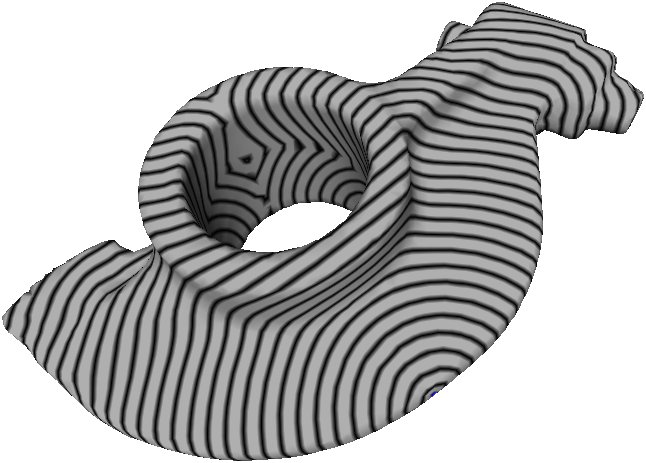
\includegraphics[width=0.9\columnwidth]{images/geodesic_rocket-arm.png}}
	\caption{Geodesic distance radius from a starting point on genus 1 rocket arm model. At the hole, we can see some sharp pattern which can be recognize as geodesic path came from different directions.}
	\label{fig:geodesic rocket arm}
\end{figure}

\subsection*{Notations}
Before explaining various algorithms of homotopy, let us define basic notations. We represent a 2-manifold triangular surface or mesh by $\mathscr{M}:=(V,F)$, where $V:=\{ v_{i}\in \mathbb{R}^3 \mid i = 1, ... , n_v\}$ is a set of $n_v$ vertices and $F:=\{ f_{i}(a,b,c) \mid a,b,c = 1, ... , n_v : a \neq b \neq c\}$ is a set of $n_f$ faces. We also define $E:=\{ e_{i}(a,b) \mid a,b = 1, ... , n_v : a \neq b\}$ as a set of $n_e$ edges found in the surface $\mathscr{M}$. We assume that the mesh has genus $g$ topology. 


\section{\uppercase{Related Works}}
\label{sec:related works}
\noindent As for a topic of topological converting in the past years, there was a novel work  by \cite{Erickson:2002:OCS:513400.513430} that studied the problem of cutting a topological surface into a disk efficiently. They have proposed a cutting method that gave some elegant theoretical guarantees. However, the algorithm is very complex to implement. It finds the shortest loop path connecting vertices to the vertex itself by using a front propagation technique, and then tests if the considering loop path reduces the surface genus or simply cuts the surface into two pieces. It has topologically-sufficient cut as $2g$ loops. The generation of minimal length cut that converts a high genus surface into a topological disk is a NP-hard problem. One method is a brute force approach which consumes a lot of time. However, it is an approximation of the shortest cut graph in $O(g^2 n \log n)$ where $n$ denotes complexity of the surface. \cite{Erickson:2005:GOH:1070432.1070581} studied about a greedy homotopy basis and improved its calculation speed in $O(n \log n)$
by using a straightforward application of Dijkstra's shortest path algorithm \cite{Dijkstra59anote}. 

From the efficiency point of view, it is important to compute non-trivial cycles on orientable surfaces. Non-trivial cycles mean non-contractible and non-separating cycles which guarantee topological surface cutting into disk. Recently, \cite{Kutz:2006:CSN:1137856.1137919} presents an algorithm that computes a shortest non-trivial cycle in $O(n \log n)$ on orientable combinatorial surface of bounded genus. The algorithm is based on universal-cover constructions to find short cycles.

There are several studies that try to define a cut graph by surface properties. A study by \cite{Patane:2007:FCB:1224804.1224947} presents an algorithm that builds up the cut graph on the iso-contours from Reeb graph which codes the topology of a given surface $\mathscr{M}$ in a combinatorial structure and generates loops together. Another study by \cite{Jin:2013:CSH:2396897.2396971}, presents an algorithm to compute the shortest homotopic loop with negative Euler characteristic based on the surface hyperbolic uniformization metric. They also demonstrate two applications: constructing extremal quasi-conformal mappings between same topology surfaces, and detecting homotopy between two paths or cycles on a surface. 

There is an iterative method called "geometry images" by \cite{Gu:2002:GI:566654.566589}, which is similar to that \cite{Dey:1994:NTC:177424.178001}. This method presents a remeshing approach using square surface parameterization to create mapping between irregular surface $\mathscr{M}$ in $\mathbb{R}^3$ domain, and square plane in $\mathbb{R}^2$ domain. To get low error on remeshing, they present how to create a cut graph from any kinds of surfaces $\mathscr{M}$ regardless from the pre-analysis of topology and boundary edges.

\begin{figure}[!h]
	%\vspace{-0.2cm}
	\centering
	\subfloat[Geometry of surface]{\label{fig:gim3d}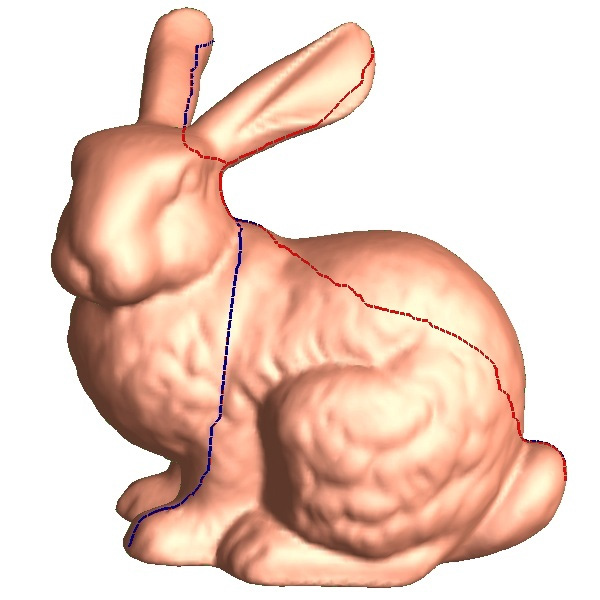
\includegraphics[width=0.45\columnwidth]{images/gim_bunny3D.png}}
	\hspace{10pt}
	\subfloat[Geometry image]{\label{fig:gim2d}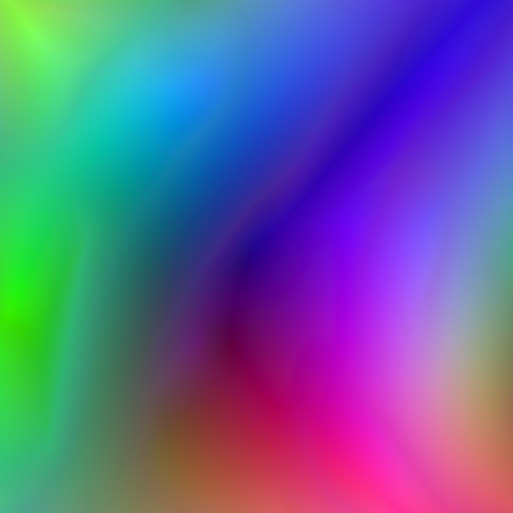
\includegraphics[width=0.45\columnwidth]{images/gim_bunny2D.png}}
	
	\caption{A geometry image.}
	\label{fig:gim figure}
\end{figure}

Since our approach is based on geometry images, we explain in section \ref{sec:previous algorithm} how it creates a cut graph for homotopy cutting on an irregular surface $\mathscr{M}$ with genus $g$.
\section{\uppercase{Previous Algorithm}}
\label{sec:previous algorithm}
\noindent The algorithm of \cite{Gu:2002:GI:566654.566589} is divided into two parts i.e., homotopy cutting and its augmentation. The augmentation aims to improve its subsequent square planar domain parameterization. We explain the first part that involves the definition of a cut graph and a converting surface $\mathscr{M}$ into disk.

\begin{figure*}[t]
	\centering		
	\subfloat[\label{fig:OriginalGenusReduceMethodStepByStep01}]{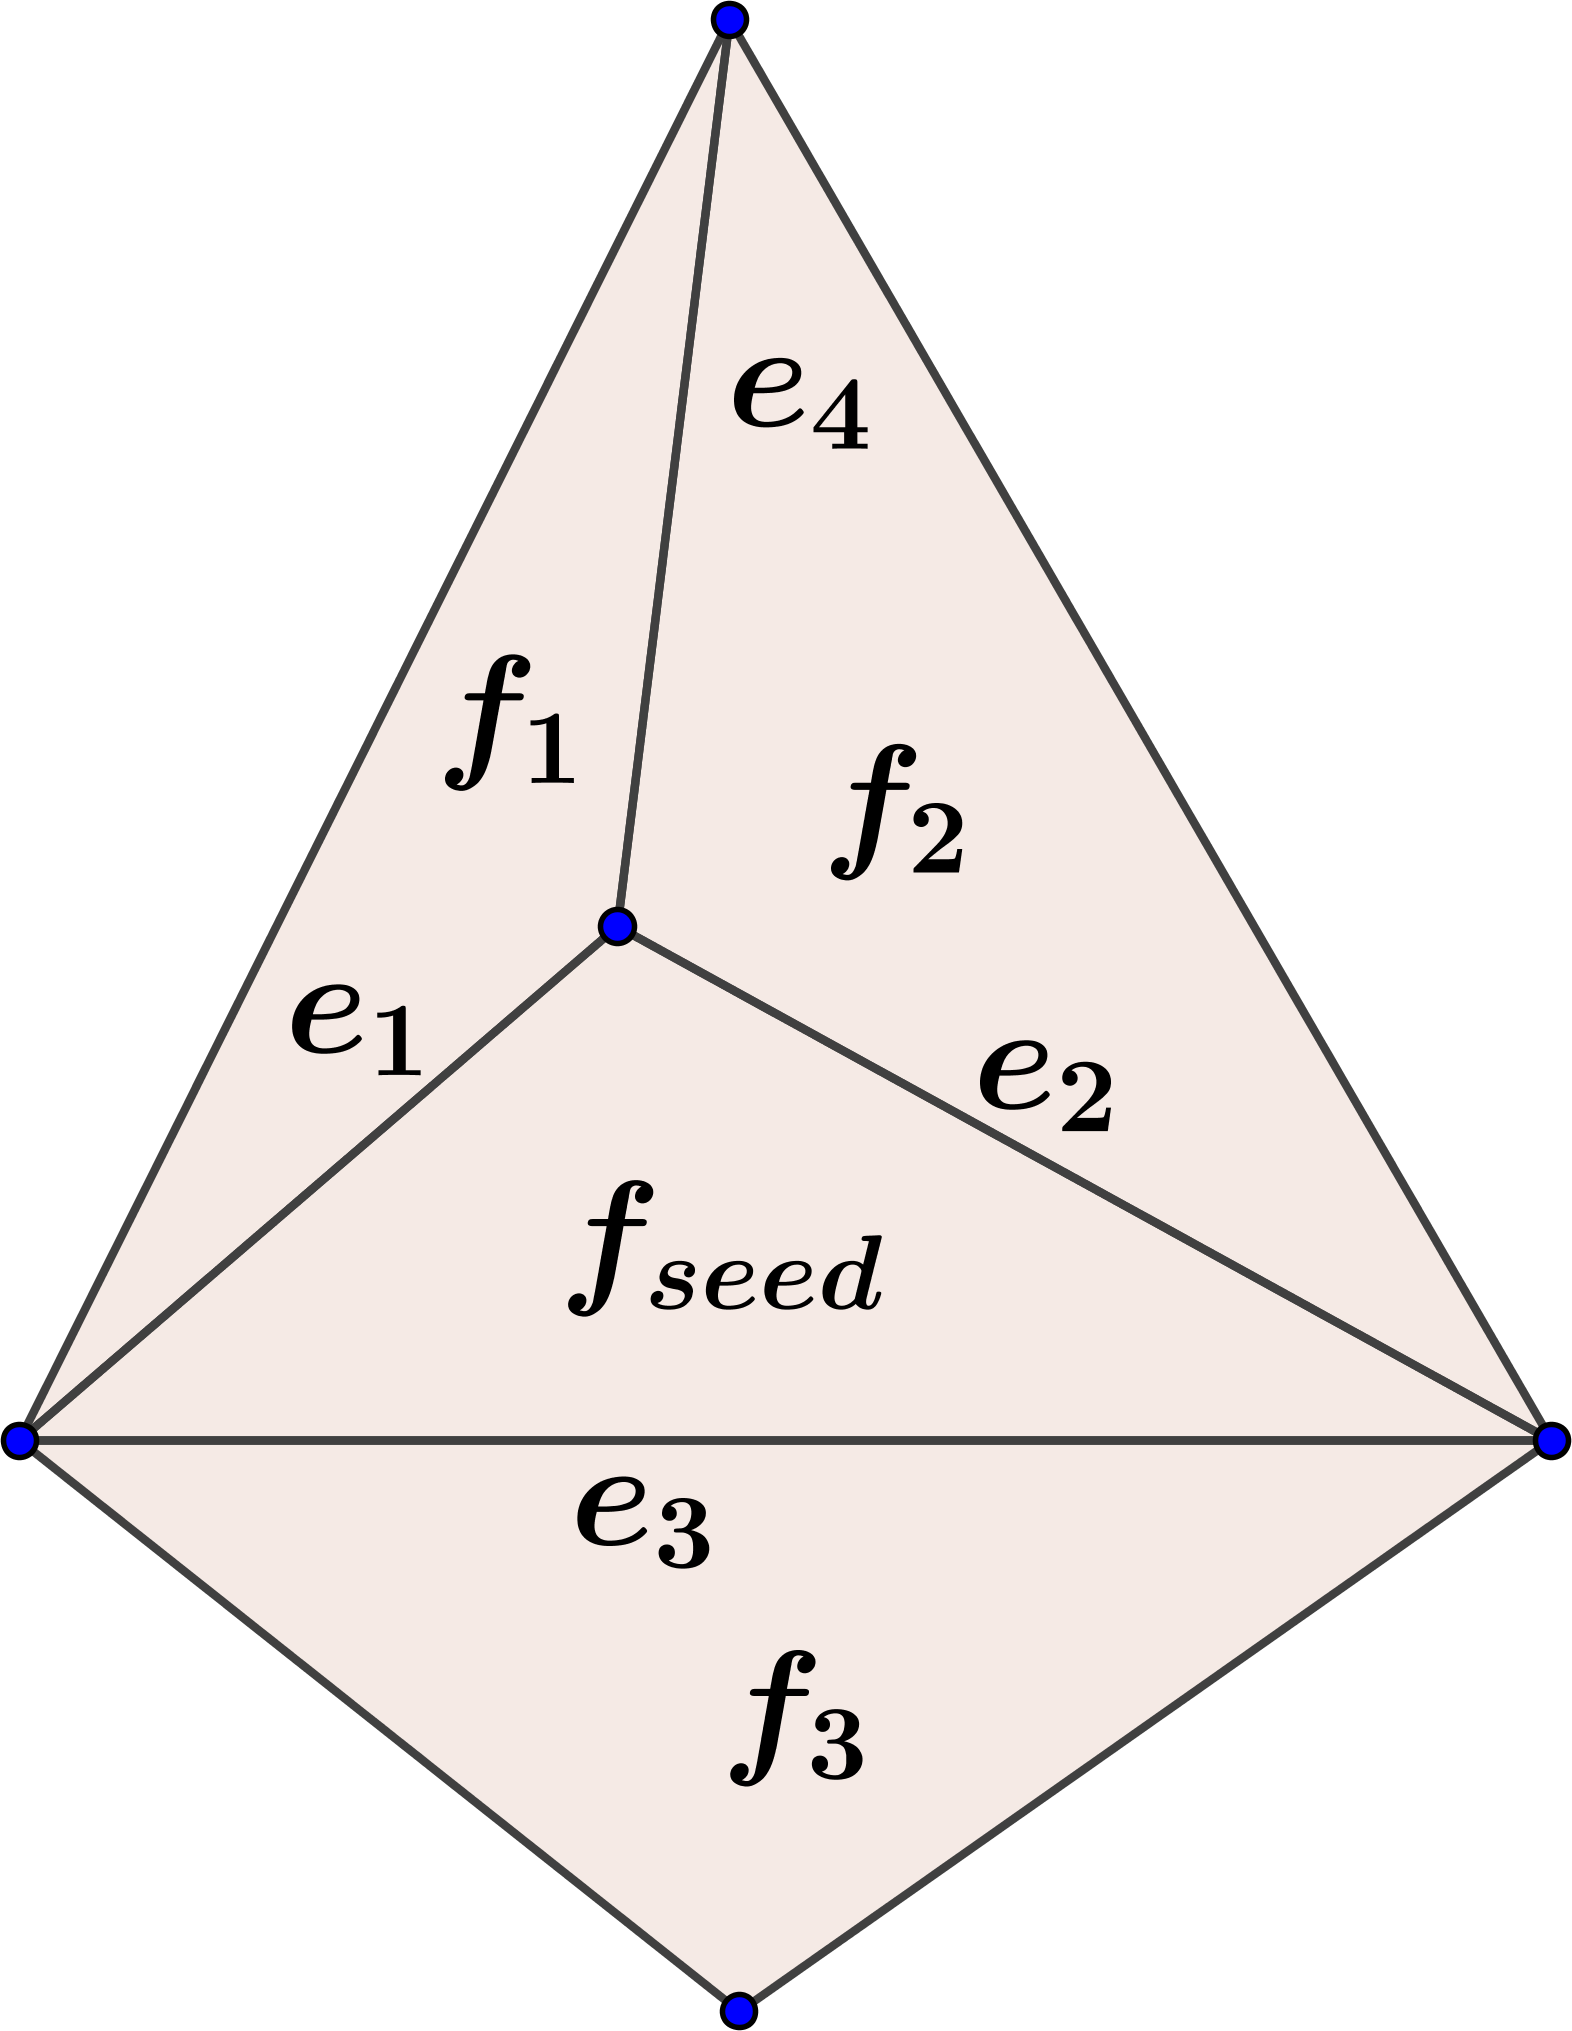
\includegraphics[width=0.175\linewidth]{images/gim_progress_01.png}}\hspace{10pt}
	\subfloat[\label{fig:OriginalGenusReduceMethodStepByStep02}]{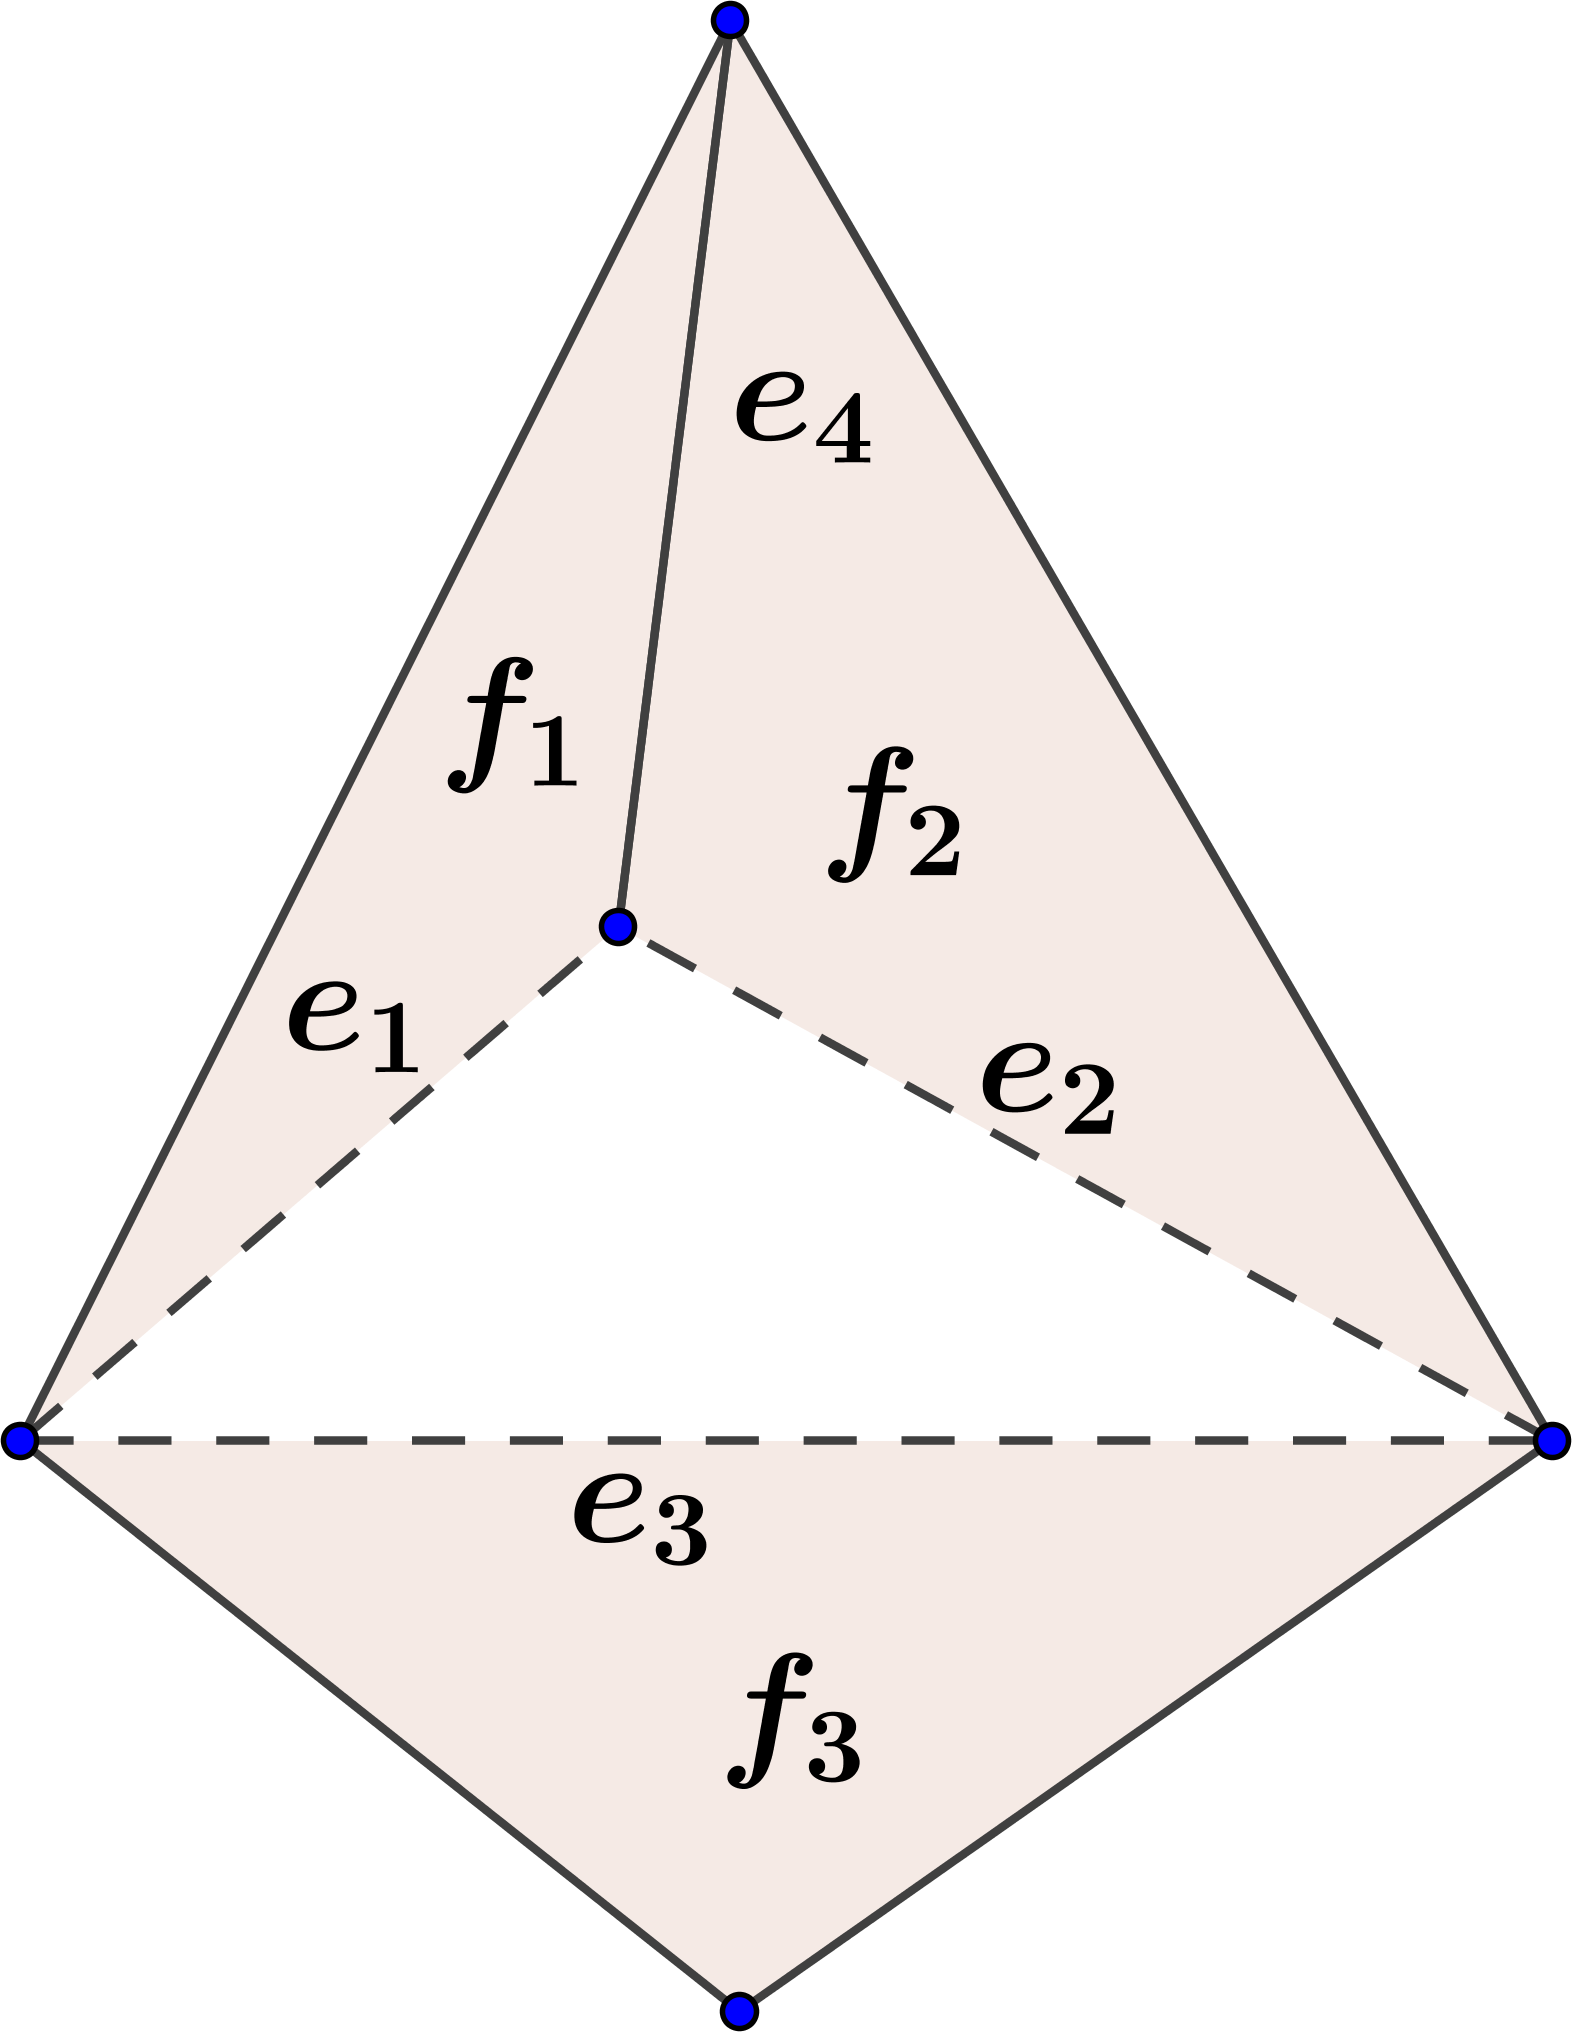
\includegraphics[width=0.175\linewidth]{images/gim_progress_02.png}}\hspace{10pt}
	\subfloat[\label{fig:OriginalGenusReduceMethodStepByStep03}]{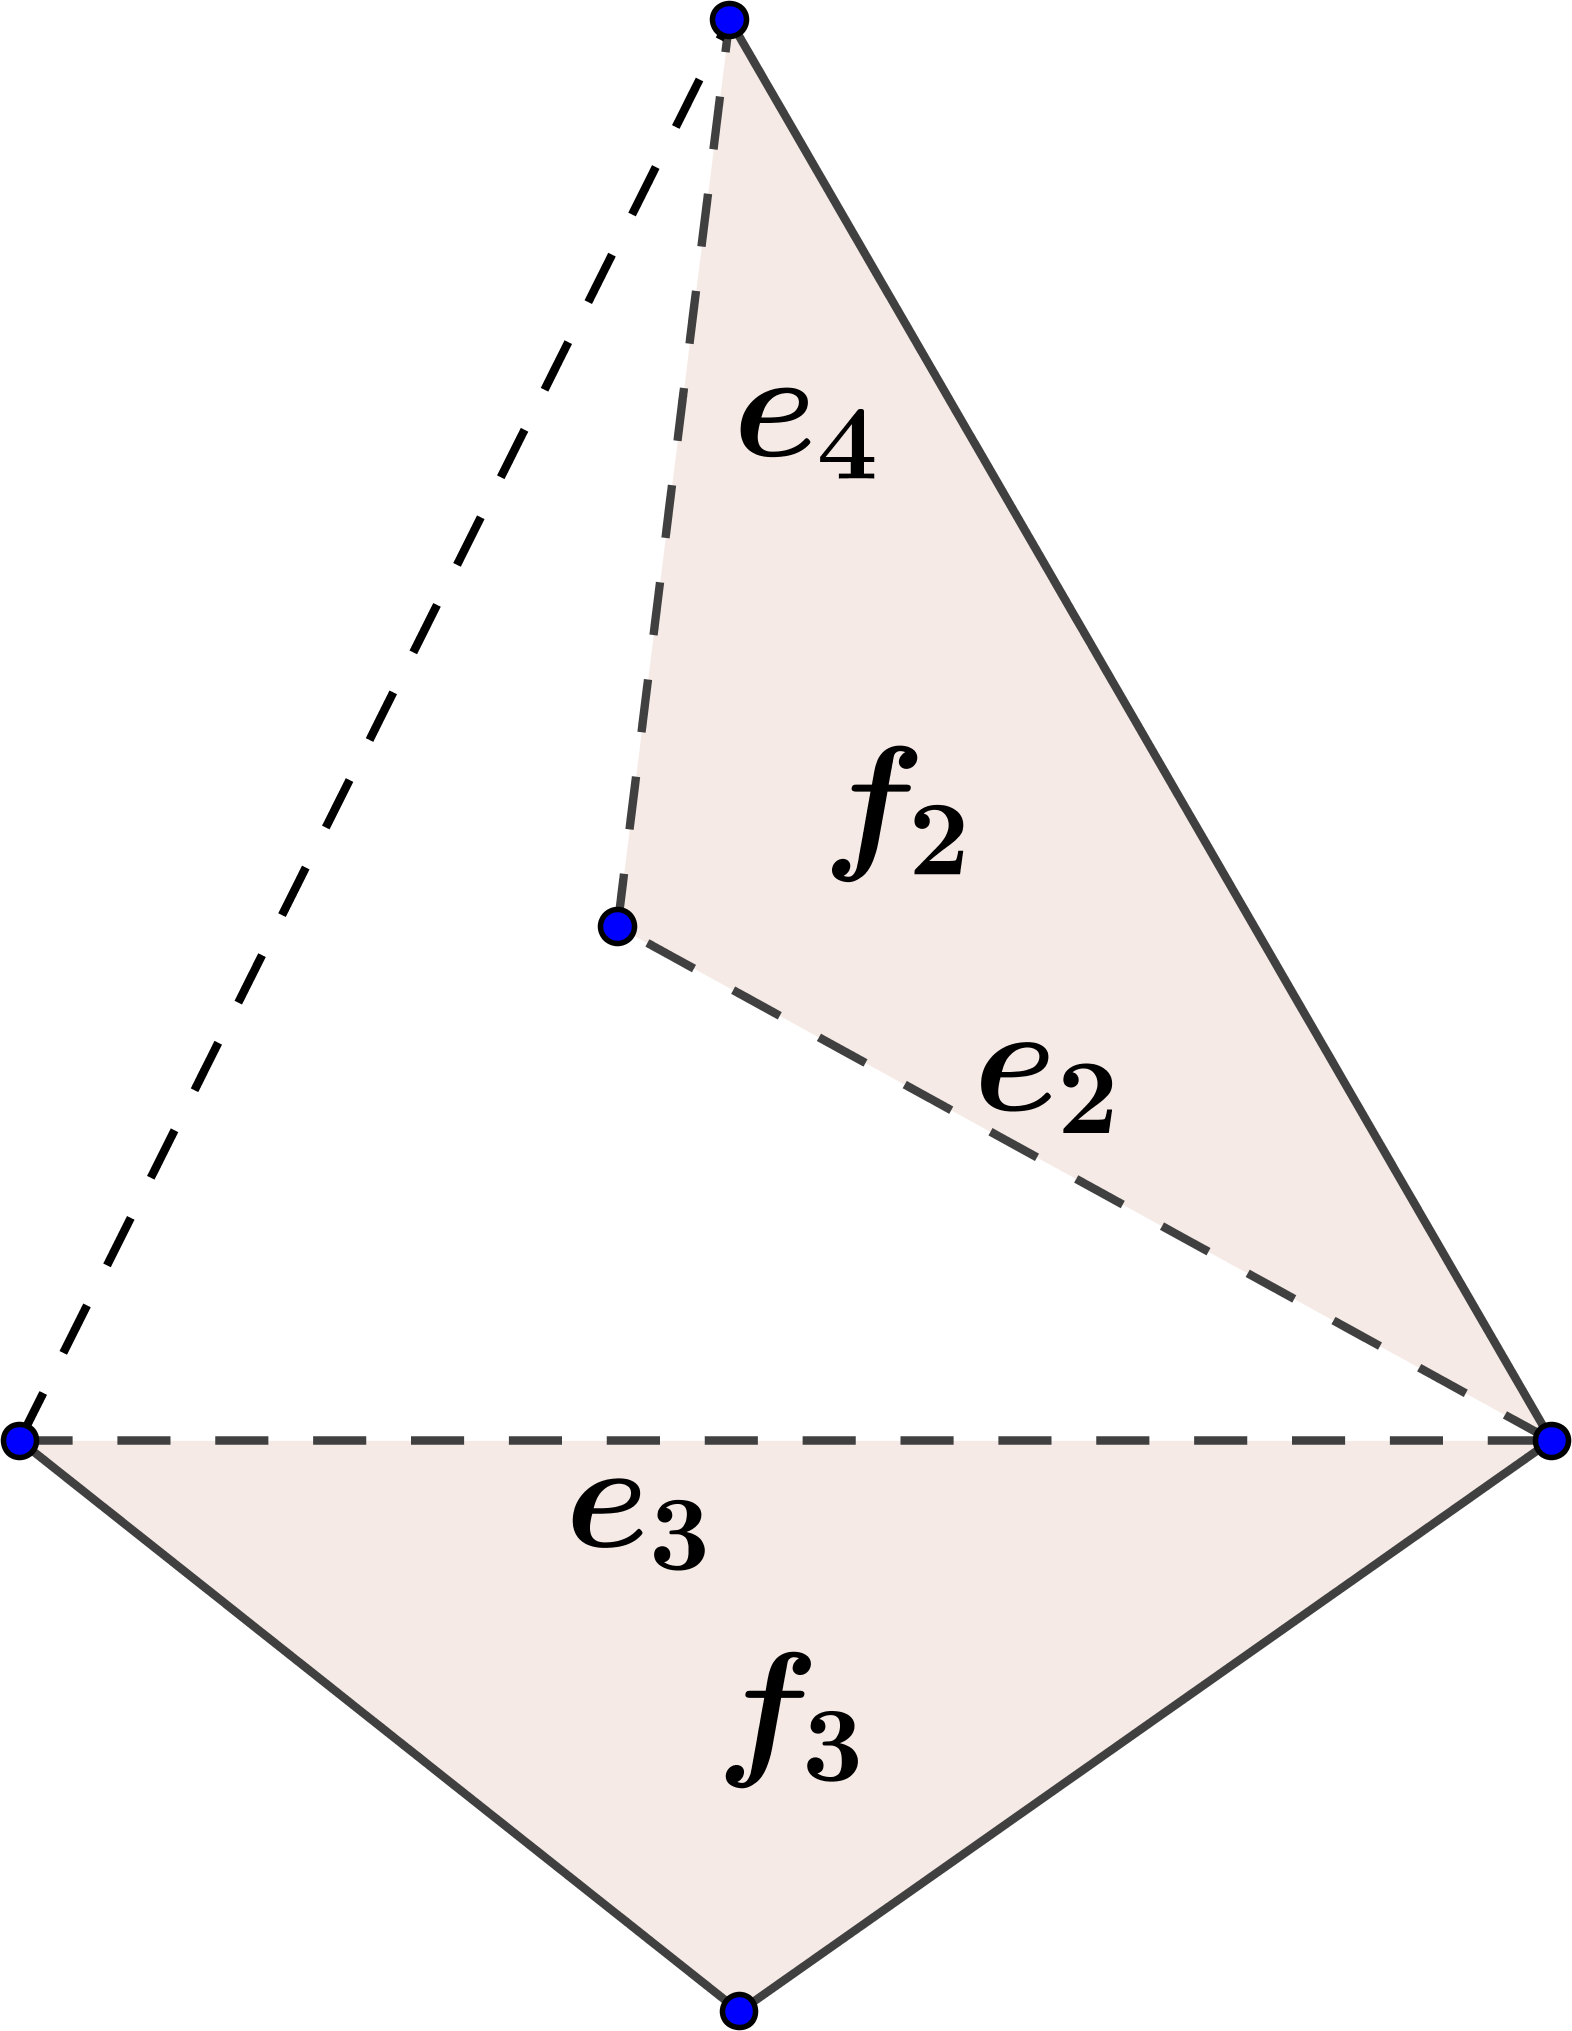
\includegraphics[width=0.175\linewidth]{images/gim_progress_03.png}}\hspace{10pt}
	\subfloat[\label{fig:OriginalGenusReduceMethodStepByStep04}]{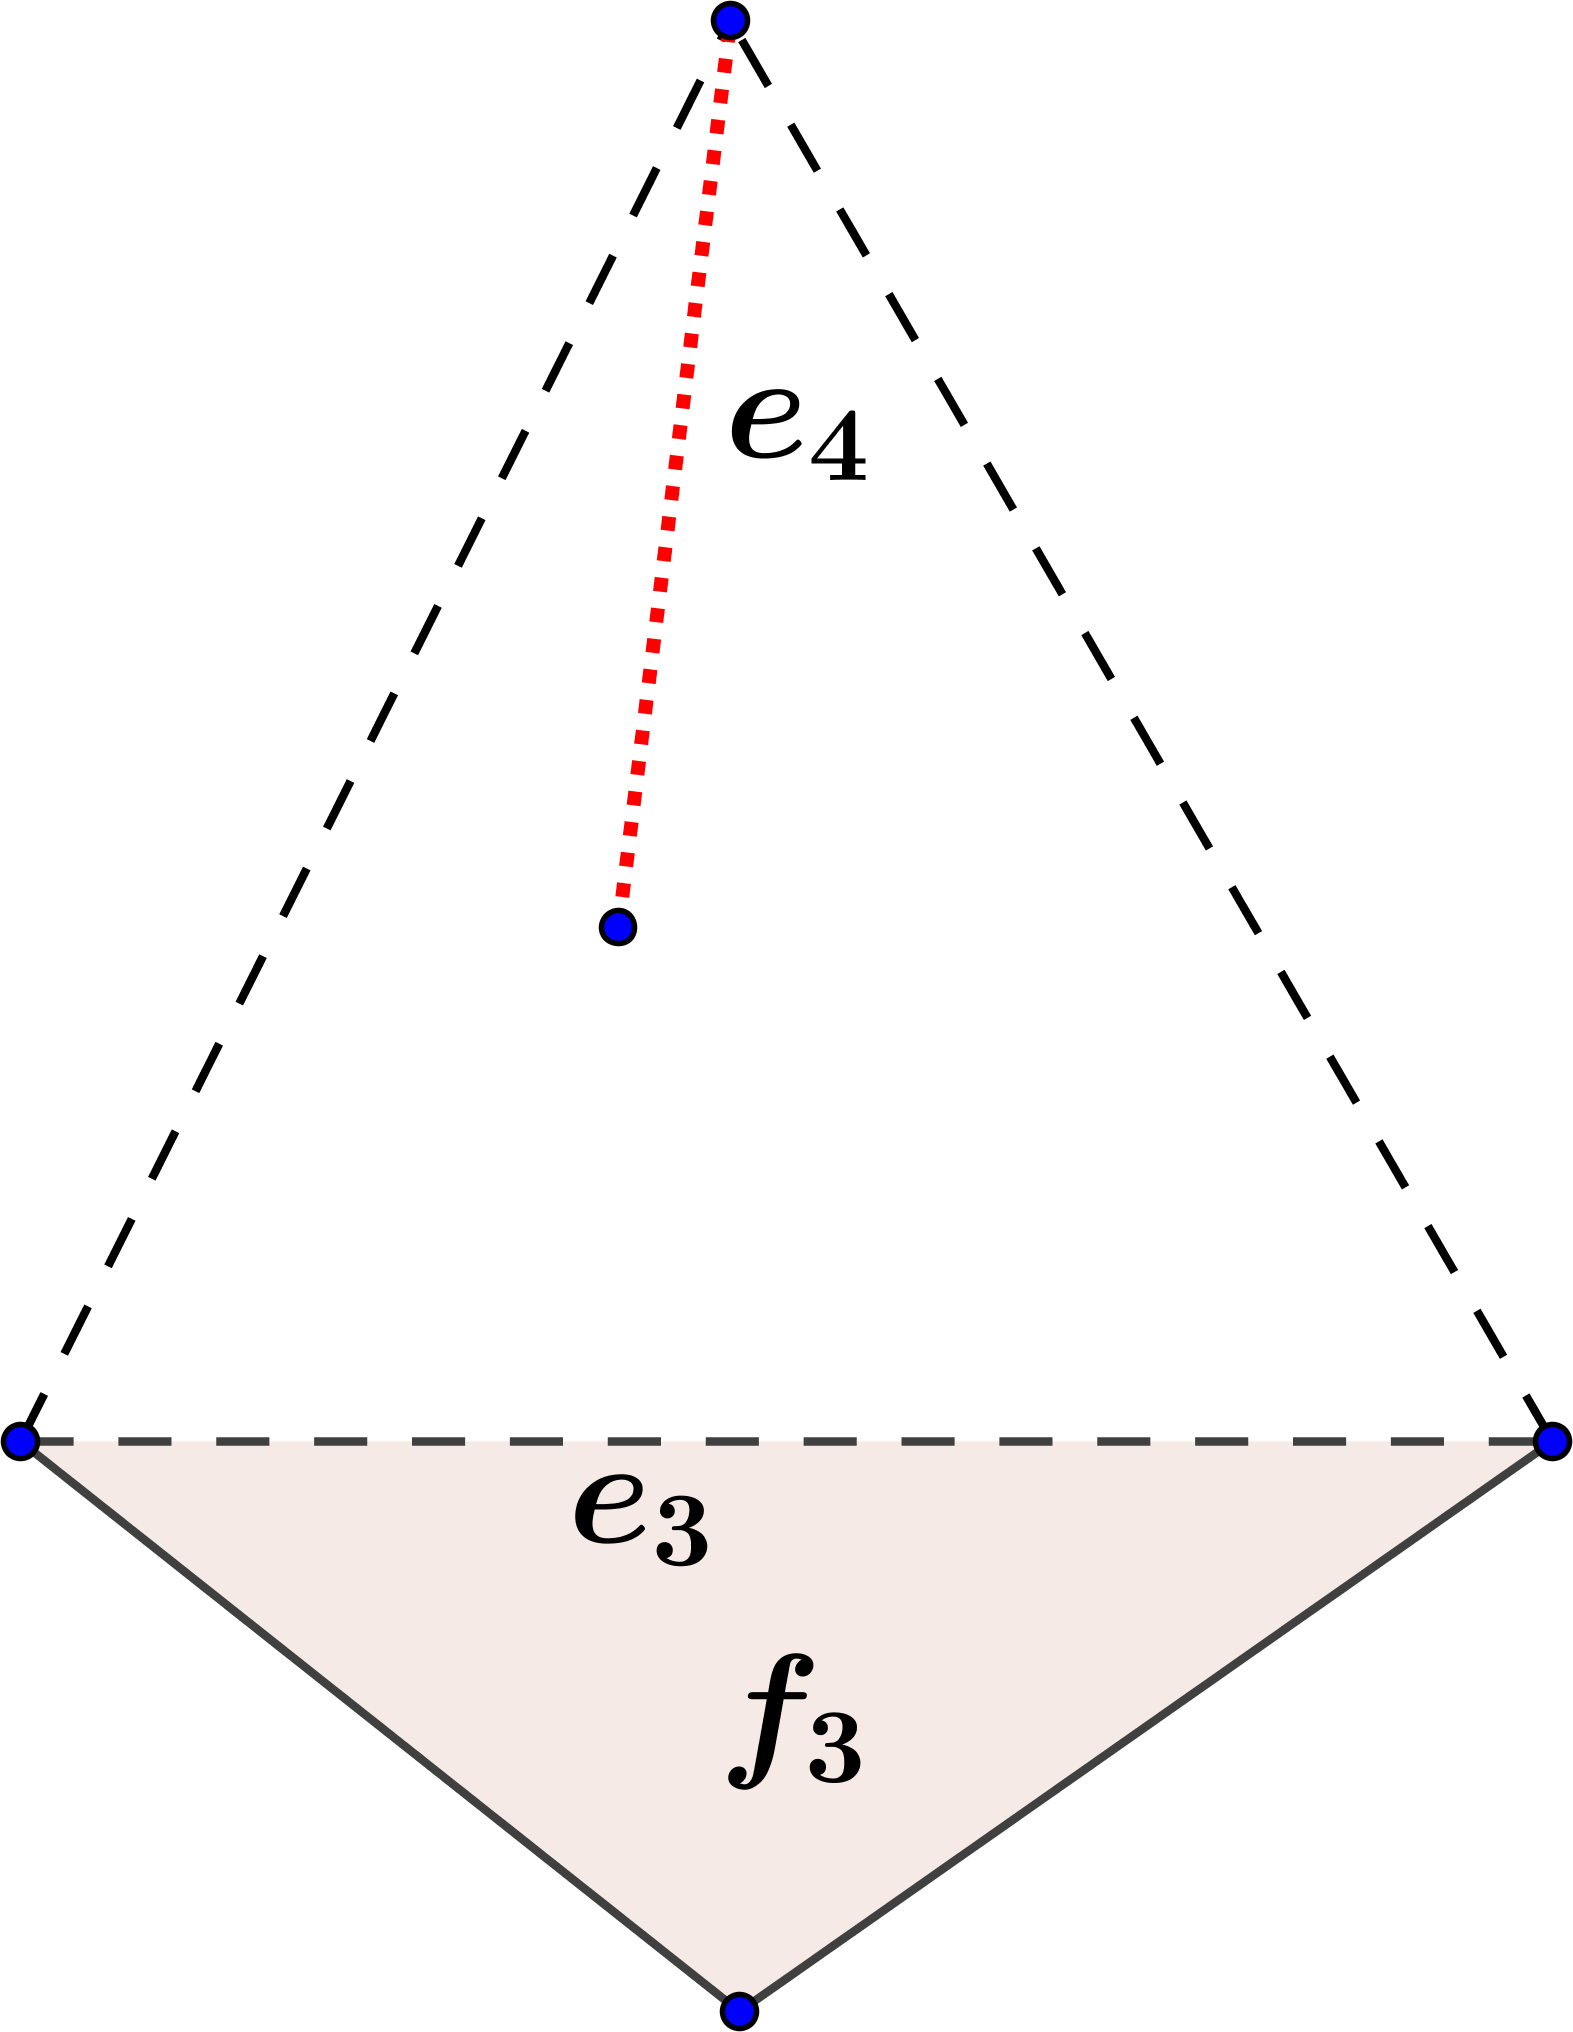
\includegraphics[width=0.175\linewidth]{images/gim_progress_04.png}}\hspace{10pt}		
	\subfloat[\label{fig:OriginalGenusReduceMethodStepByStep05}]{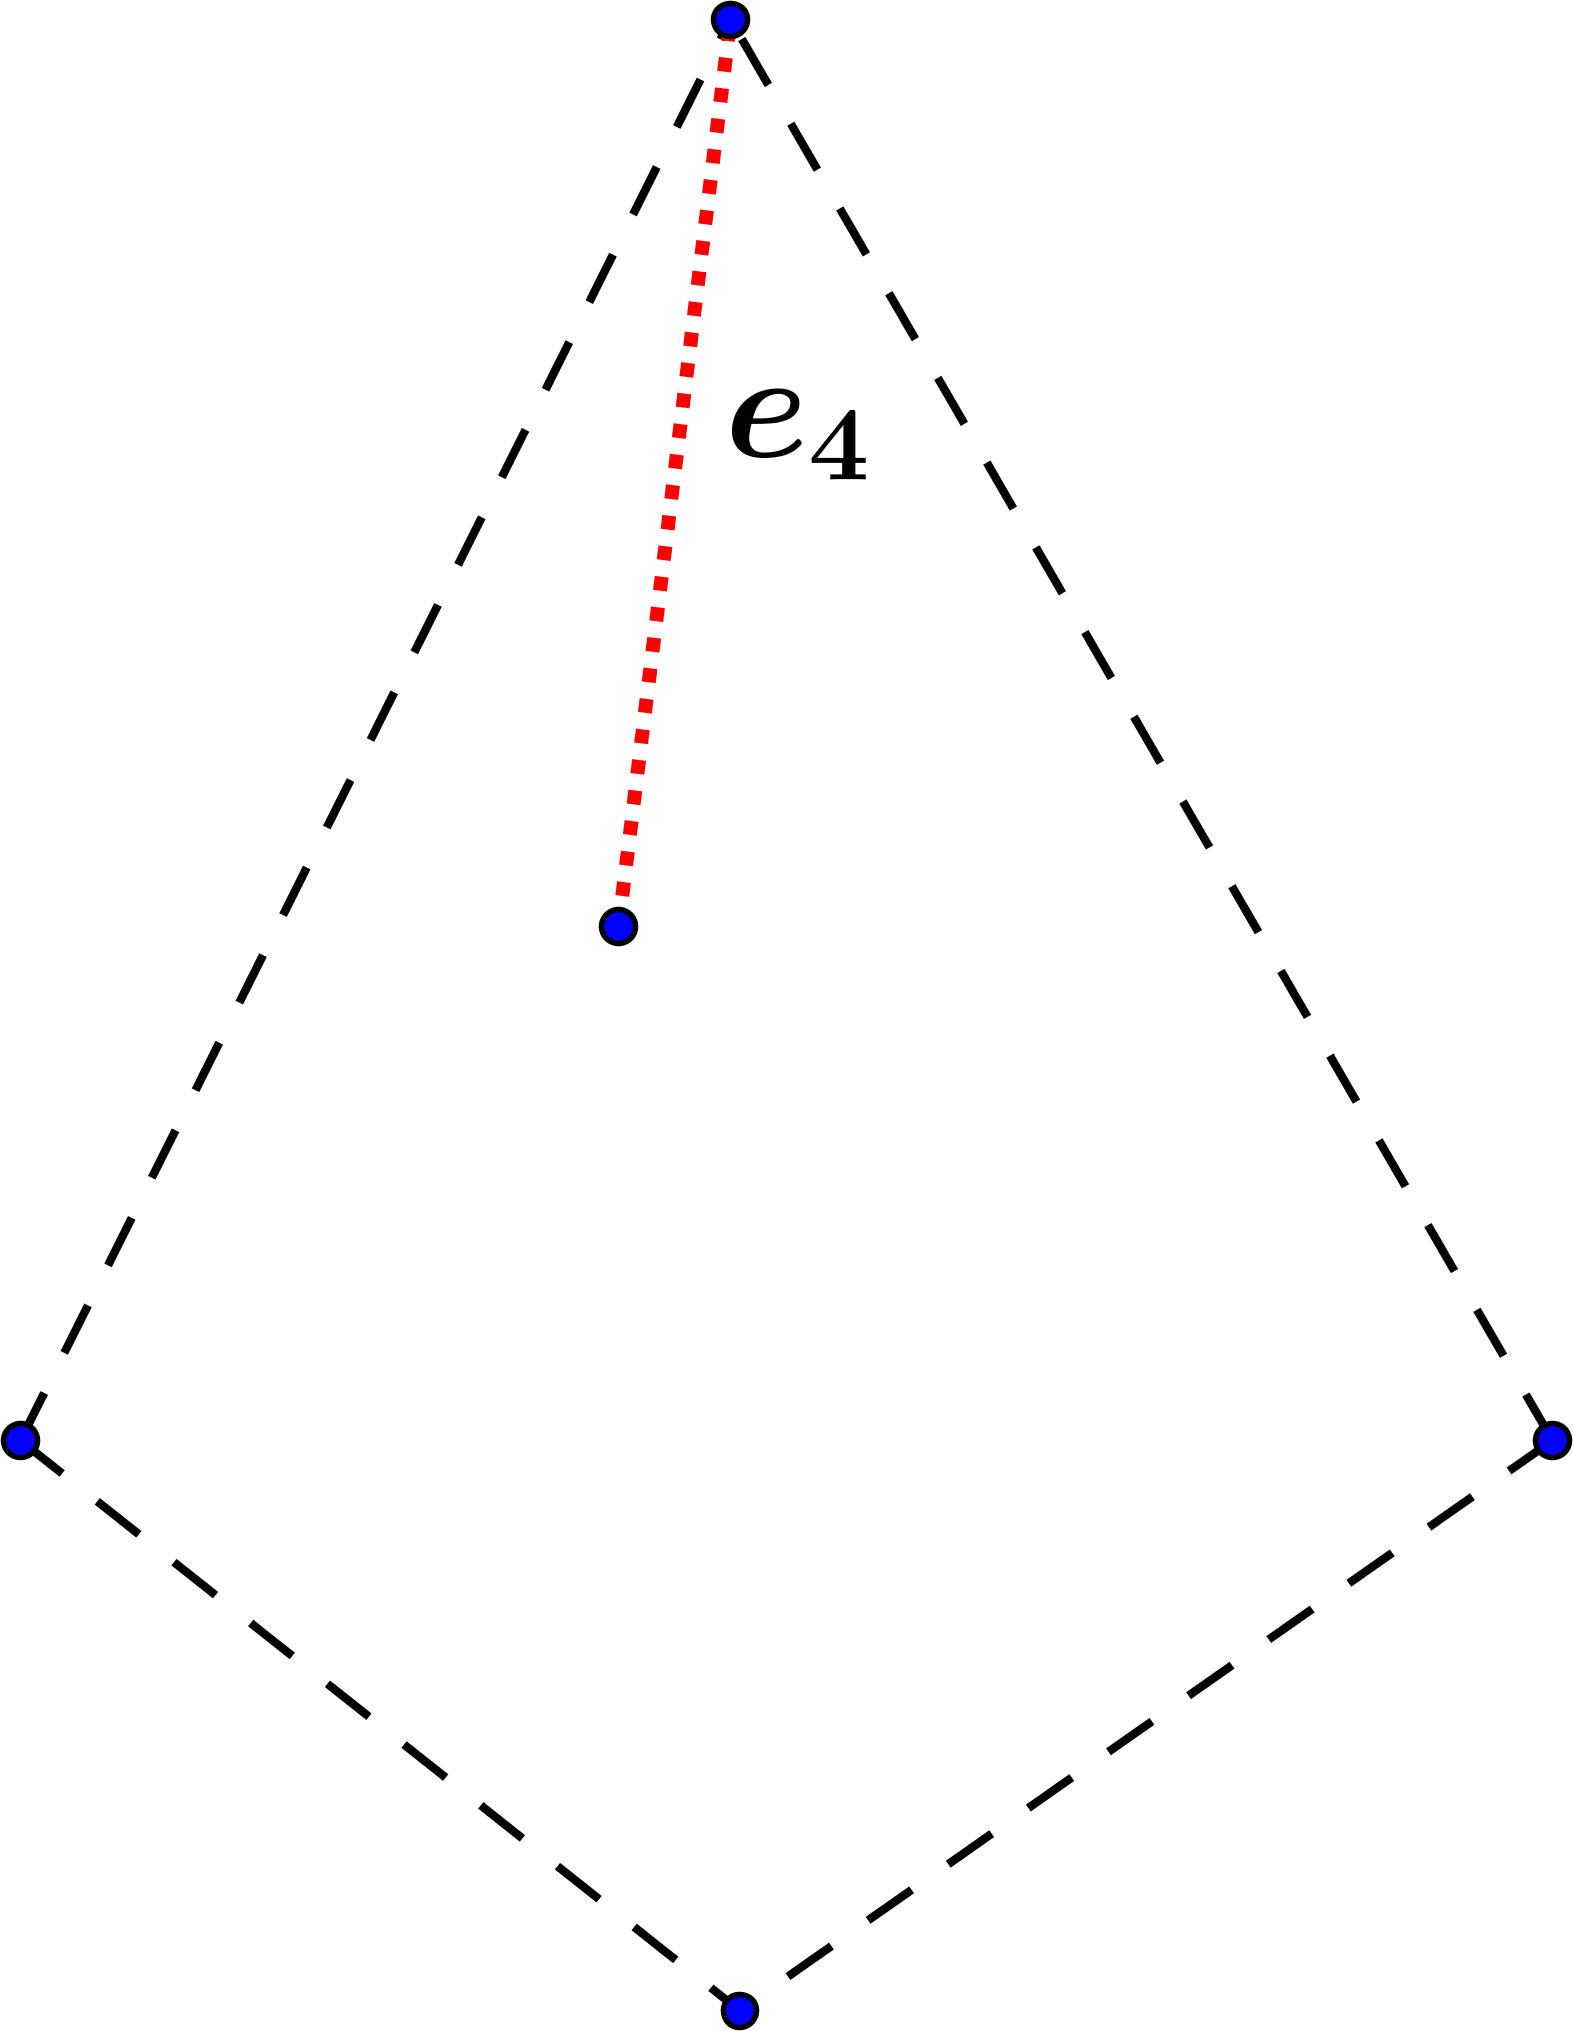
\includegraphics[width=0.175\linewidth]{images/gim_progress_05.png}}
	\caption{Processes from removing a seed triangle from a mesh. Dash lines mean edges that are adjacent to only one triangle at the moment. \subref{fig:OriginalGenusReduceMethodStepByStep01} shows before removing stage. \subref{fig:OriginalGenusReduceMethodStepByStep02} shows after removing the seed triangle; that is, edges $e_1$,$e_2$ and $e_3$ are adjacent to only one triangle. Assume that geodesic distance from $f_{seed}$ to $e_1$ is the smallest. \subref{fig:OriginalGenusReduceMethodStepByStep03} shows the result of removing edge $e_1$ and face $f_1$. The edge $e_4$ become the one that adjacent to only one triangle. Let $e_2$ is next smallest geodesic distance. \subref{fig:OriginalGenusReduceMethodStepByStep04} shows the result of removing $e_2$ and $f_2$. The edge $e_4$ becomes a candidate of cut graph edge (red dot line). \subref{fig:OriginalGenusReduceMethodStepByStep05} shows the result of next step that removing $e_3$ and $f_3$.}
	\label{fig:OriginalGenusReduceMethodStepByStep}
\end{figure*}

At the beginning in the method , if the mesh has boundaries, let $\mathscr{B}$  be the set of original boundary edges that remain unchanged in the whole process and will be included in final cut graph ${\rho}$. It first starts by removing a single seed triangle from the mesh. At this moment, each edge of the seed triangle is adjacent to only one triangle respectively (see figure \subref*{fig:OriginalGenusReduceMethodStepByStep02}).  After removing the seed triangle from the mesh, there are two processing phases.

In the first phase, it repeatedly detects an edge adjacent exactly to one triangle that is not in $\mathscr{B}$, and removes both the edge and the triangle from the mesh structure. The rest two edges are left (see figure \subref*{fig:OriginalGenusReduceMethodStepByStep03}). If the rest edges of the removing triangle are not adjacent to any triangle, then the edges will become one of candidates of cut graph (see figure \subref*{fig:OriginalGenusReduceMethodStepByStep04}). Generally, removing one edge and one triangle triggers more two edges to be adjacent to only one triangle further. Because of the above condition, the removing propagation will keep spreading out from the seed triangle according to geodesic distance in order to get minimum radius result. Since a 2-manifold triangle mesh is being processed, any triangle will be removed eventually. Therefore, this phase ends when there is no triangle left and there remain only edges and their vertices as candidate cut graph edges (see figure \subref*{fig:fig-original_genus_reducing_process-c}). At this point, the cut $\rho$ consists of a set of connecting $2g$ loops.

In the second phase, we again iteratively detect a valence-1 vertex and its corresponding edge, and remove both the vertex and the edge (see figure \ref{fig:fig-original_remove_dangling_edges_step_by_step}). The purpose of this phase is to remove unnecessary dangling edges remained in the first phase. The dangling edges will be repeatedly trimmed away until there is no valence-1 vertex left in the cut $\rho$. There are only edges that form connected loops as a cut graph in the cut $\rho$. At last, all loops in $\rho$ are straightened by computing a local shortest path in each loop. Finally, the connected $2g$ loop cut graph in $\rho$ is homotopy basis: a cut graph that converts the surface into a topological disk patch. See figure \ref{fig:fig-original_genus_reducing_process} for overall process of finding graph cut on a genus-3 mesh.



For the case of closed surface of genus 0, the overall processes from this part will generate the cut $\rho$ that consists of only one vertex. To be able to map into planar domain, we add two adjacent edges of the vertex into the cut graph $\rho$. On the other hand, for the case of a mesh having one or more holes, it will result in connected graphs between any two holes.

\begin{figure}[h!]
	\centering		
	\subfloat[\label{fig:fig-original_remove_dangling_edges_step_by_step-a}]{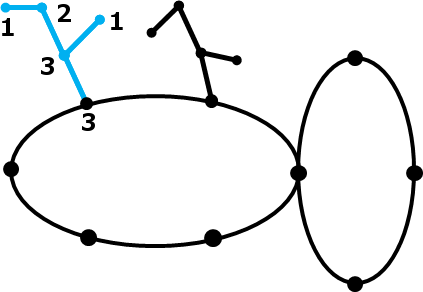
\includegraphics[width=0.45\columnwidth]{images/fig-original_remove_dangling_edges_step_by_step-a.png}} \hspace{10pt}
	\subfloat[\label{fig:fig-original_remove_dangling_edges_step_by_step-b}]{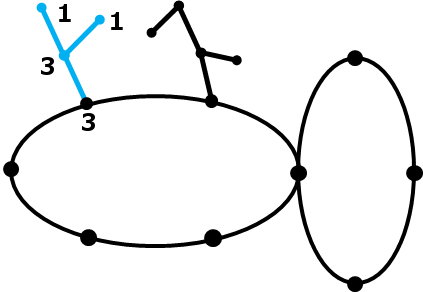
\includegraphics[width=0.45\columnwidth]{images/fig-original_remove_dangling_edges_step_by_step-b.png}}\\		
	\subfloat[\label{fig:fig-original_remove_dangling_edges_step_by_step-c}]{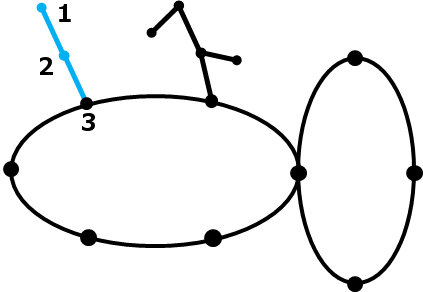
\includegraphics[width=0.45\columnwidth]{images/fig-original_remove_dangling_edges_step_by_step-c.png}}	\hspace{10pt}	
	\subfloat[\label{fig:fig-original_remove_dangling_edges_step_by_step-d}]{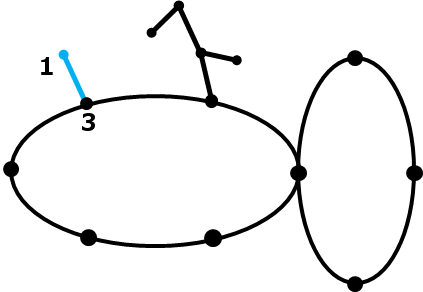
\includegraphics[width=0.45\columnwidth]{images/fig-original_remove_dangling_edges_step_by_step-d.png}}	\\
	\subfloat[\label{fig:fig-original_remove_dangling_edges_step_by_step-e}]{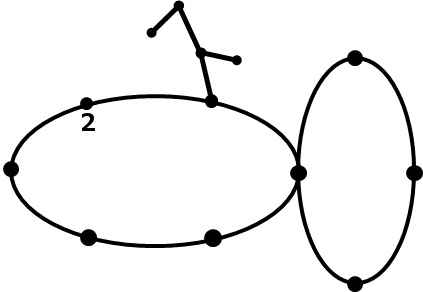
\includegraphics[width=0.45\columnwidth]{images/fig-original_remove_dangling_edges_step_by_step-e.png}}	\hspace{10pt}
	\subfloat[\label{fig:fig-original_remove_dangling_edges_step_by_step-f}]{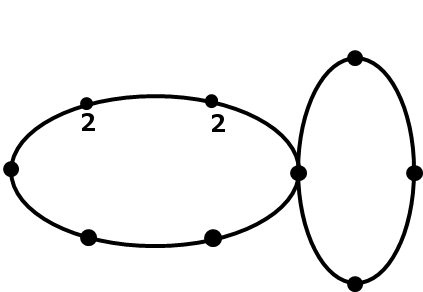
\includegraphics[width=0.45\columnwidth]{images/fig-original_remove_dangling_edges_step_by_step-f.png}}	 
	\caption[]{Process on removing dangling edges. The numbers on vertices indicate present valence number. We focus on the removing of blue dangling edges. \subref{fig:fig-original_remove_dangling_edges_step_by_step-a} shows initial state where there are two valence-1 edges. \subref{fig:fig-original_remove_dangling_edges_step_by_step-b} - \subref{fig:fig-original_remove_dangling_edges_step_by_step-d} show the following steps that remove valence-1 edge along with its vertex. \subref{fig:fig-original_remove_dangling_edges_step_by_step-e} shows that all blue dangling edges have been removed. \subref{fig:fig-original_remove_dangling_edges_step_by_step-f} shows the process of removing other dangling edges until valence-1 edge has not been found in graph.}
	\label{fig:fig-original_remove_dangling_edges_step_by_step}
\end{figure}


\begin{figure}[h!]
	\centering		
	\subfloat[\label{fig:fig-original_genus_reducing_process-a}]{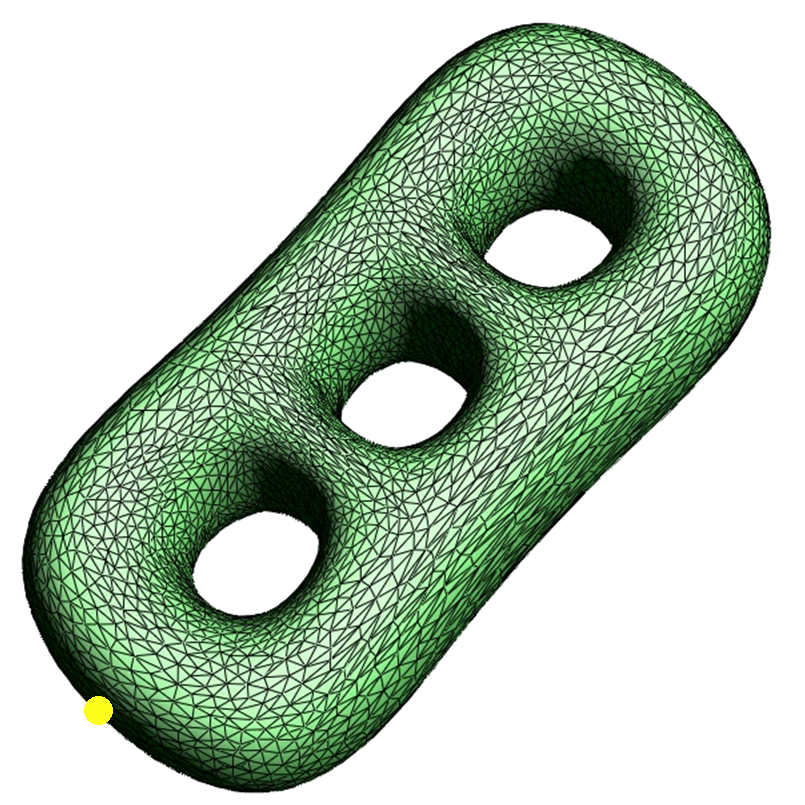
\includegraphics[width=0.31\columnwidth]{images/fig-original_genus_reducing_process-a.png}}
	\hspace{0.00\columnwidth}
	\subfloat[\label{fig:fig-original_genus_reducing_process-b}]{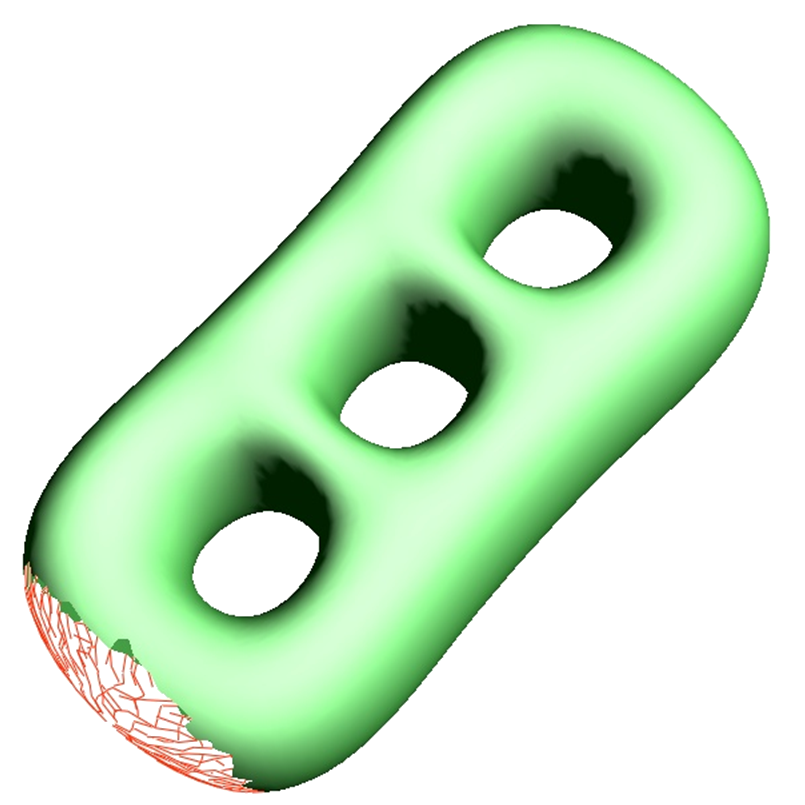
\includegraphics[width=0.31\columnwidth]{images/fig-original_genus_reducing_process-b.png}}
	\hspace{0.00\columnwidth}
	\subfloat[\label{fig:fig-original_genus_reducing_process-c}]{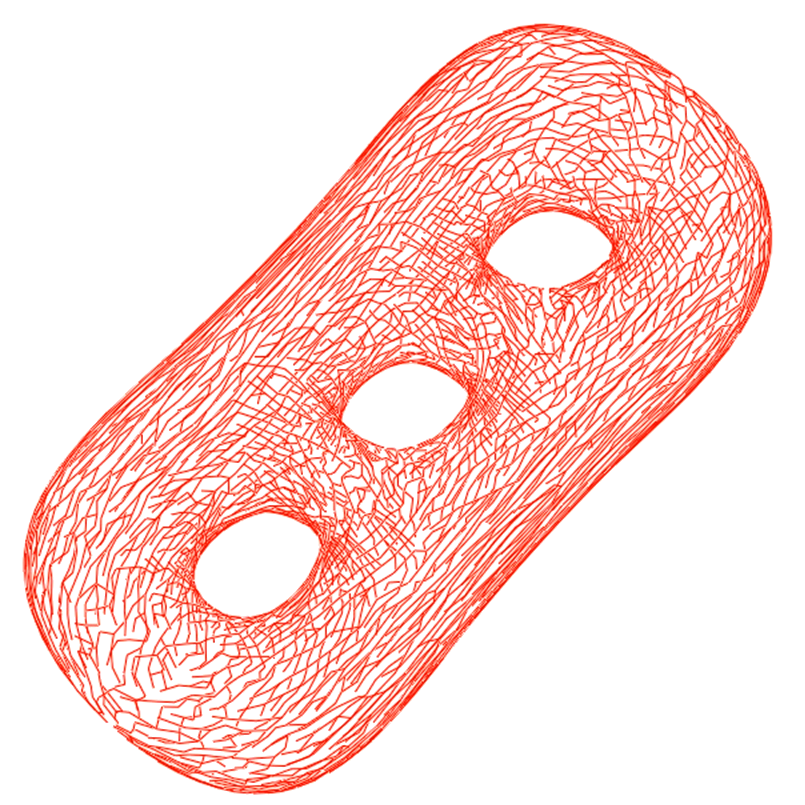
\includegraphics[width=0.31\columnwidth]{images/fig-original_genus_reducing_process-c.png}}
	\hspace{0.00\columnwidth}
	\subfloat[\label{fig:fig-original_genus_reducing_process-d}]{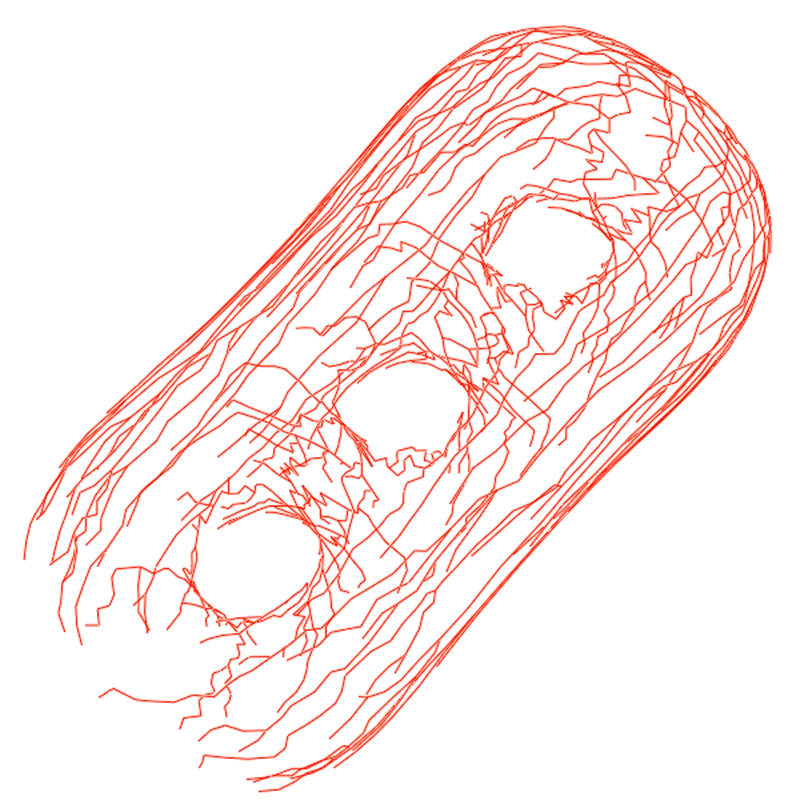
\includegraphics[width=0.31\columnwidth]{images/fig-original_genus_reducing_process-d.png}}
	\hspace{0.00\columnwidth}
	\subfloat[\label{fig:fig-original_genus_reducing_process-e}]{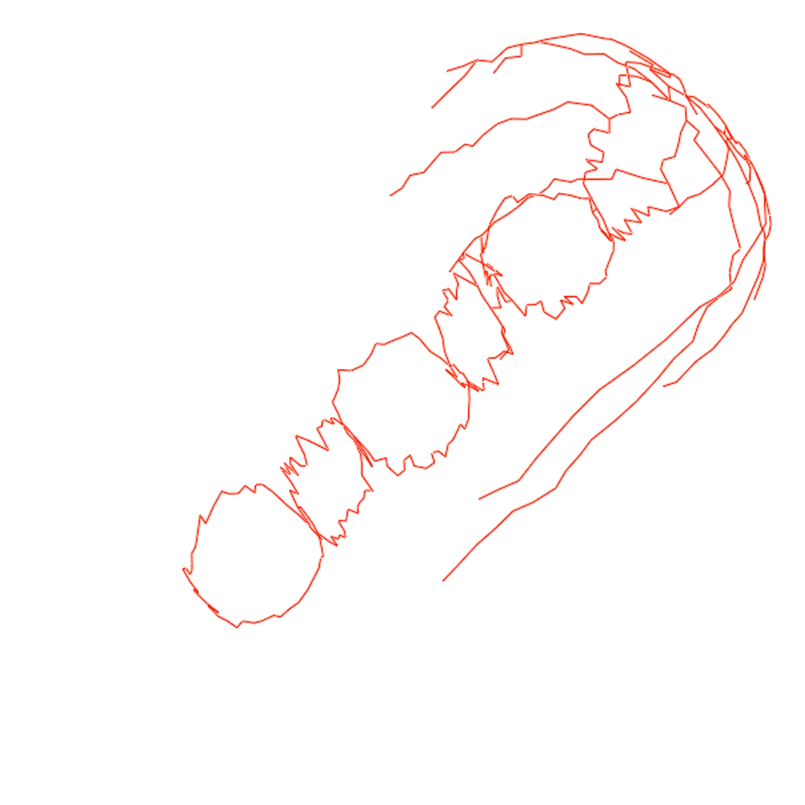
\includegraphics[width=0.31\columnwidth]{images/fig-original_genus_reducing_process-e.png}}
	\hspace{0.00\columnwidth}
	\subfloat[\label{fig:fig-original_genus_reducing_process-f}]{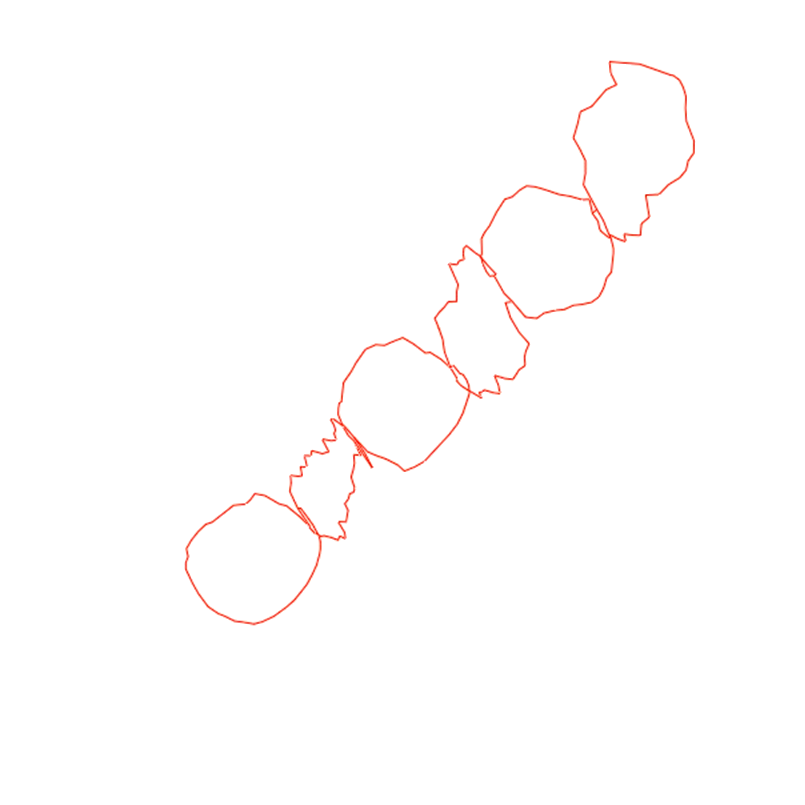
\includegraphics[width=0.31\columnwidth]{images/fig-original_genus_reducing_process-f.png}}
	\caption[]{Process of genus-reduce cutting by sequentially removing triangles, edges and vertices. \subref{fig:fig-original_genus_reducing_process-a} shows a closed genus-3 mesh with one seed triangle (yellow dot). \subref{fig:fig-original_genus_reducing_process-b} shows the intermediate state of mesh when removing triangles and edges that are adjacent to only one triangle. \subref{fig:fig-original_genus_reducing_process-c} shows edge skeleton mesh after removing all triangles. \subref{fig:fig-original_genus_reducing_process-d} and \subref{fig:fig-original_genus_reducing_process-e} show the intermediate state of mesh when removing edges and vertices that are adjacent to only one edge. \subref{fig:fig-original_genus_reducing_process-f} shows final result of straightened cutting edges after removing edges and vertices.}
	\label{fig:fig-original_genus_reducing_process}
\end{figure}

\section{\uppercase{Geodesic Distance}}
\label{sec:geodesic distance}
\noindent The algorithm by \cite{Gu:2002:GI:566654.566589} creates front propagation on geodesic distance. We consider an exact geodesic distance proposed by \cite{Mitchell:1987:DGP:33367.33372} as knows as MMP algorithm. It computes exact shortest paths on a triangular mesh. These paths typically cut across faces in the mesh, which is different from typical Dijkstra shortest paths \cite{Dijkstra59anote} that run across edges in the mesh.

\begin{figure}[!h]
	%\vspace{-0.2cm}
	\centering
	{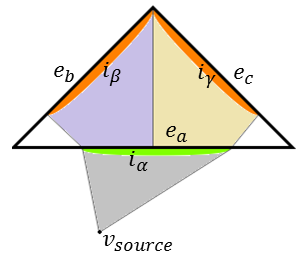
\includegraphics[width=0.75\columnwidth]{images/mmp_algorithm.png}}
	\caption{Propagation scheme of MMP algorithm: interval $i_{\alpha}$ on edge $e_a$ propagates distance pencil paths across an adjacent face to adjacent edges $e_b$ and $e_c$ }
	\label{fig:mmp algorithm}
\end{figure}

MMP algorithm creates a geodesic path for "single source and all destinations" scheme. The algorithm computes a set of intervals of each edge. An interval represents accessible pencil of lines from its pseudo-source. Each internal also acts as a pseudo-source to propagate across faces of the rest of mesh. The algorithm propagates the distance information out from the source in a Dijkstra-like fashion which can traceback any positions on mesh to the source.

The performance of MMP algorithm : They prove a worst case
running time of $O(n^2 \log n)$ when $n$ is the number of mesh edges. However in practical calculation, it can achieve on 100K triangles mesh within a few seconds. Also there is an approximate version of MMP algorithm proposed by \cite{Surazhsky:2005:FEA:1073204.1073228} that can speed up the calculation by trying to merge an interval with an adjacent intervals on the same edge before starting the propagation.

\subsection*{Notations}
After calculating exact geodesic distance from a vertex $v_s$, each edge $e_i$ that is not a boundary one, has a set of $m$ intervals $I_{e_i}:=\{ i_{e_{i,j}}(f_p,e_p,D) \mid i = 1, ... ,n_v , j = 1,...,m\}$, where $f_p$ represents the face where propagation of interval's pseudo-source across and $e_p$ represents the edge that has interval's pseudo-source. $D$ represents another informations about geodesic distance of considering interval.

\section{\uppercase{Our Approach}}
\label{sec:our approach}
\noindent Given a triangular 2-manifold mesh $\mathscr{M}$ without any topological information about genus $g$, we adopt a geometry image method \cite{Gu:2002:GI:566654.566589} to define $2g$ cut loop graph for homotopy basis. Instead of having a cut graph along the propagation by geodesic distance criteria, we try to have a cut graph in the area where it has the same geodesic distance but its pseudo-sources come from different edges.

To define such area, we calculate the exact geodesic distance from a source vertex $v_{s}$ by MMP algorithm \cite{Mitchell:1987:DGP:33367.33372} then  analyze the set of intervals in each edge $e_i$. First, we define edges whose intervals have pseudo-sources laid on both side of adjacent faces. However, this case typically can detect few edges and cannot cover all areas where the cut graph should exist. Second, we define remaining edges whose intervals cannot be a pseudo-source of adjacent edges. We define these two specific characteristic edges as a set of edges $\tilde{E}$. At this point, $\tilde{E}$ contains a lot of unnecessary dangling edges. Therefore, we eliminate them from $\tilde{E}$ by same approach in original method.

We ensure that the cut graph has non-separating cycles by considering neighbor edges of $\tilde{E}$. We define a set of neighbor edges as $\hat{E}$, 
then the candidate cut graph edges can be given by $\rho \equiv (\tilde{E} \cup \hat{E})$, and the rest edges $\acute{E}$ are given as $\acute{E} \equiv (E - \rho)$. However, $\rho$ may contain contractible cycles too. Therefore, we again need to define non-separating and non-contractible cycles from $\rho$. We follow similar basis from original method by removing an edge adjacent exactly to one triangle. However, we create priority of removing edges in queue according to $\acute{E}$,  $\hat{E}$ and $\tilde{E}$. From this point, we follow the remaining original processes: removing dangling edges and shorten loop.

We explain in details how to define the set $\tilde{E}$ and how to ensure the generation of non-separating and non-contractible cut graph.

\begin{figure}[h!]
	\centering		
	\subfloat[\label{fig:geodesic_both_face}from both sides type]{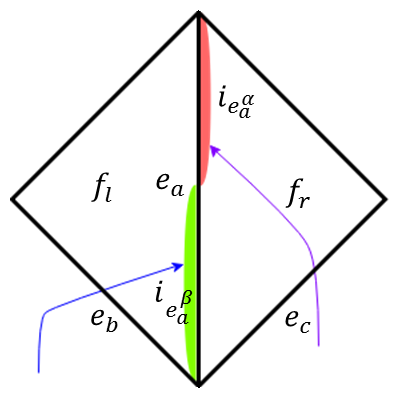
\includegraphics[width=0.49\columnwidth]{images/two_pseudosource.png}}
	\hspace{0pt}
	\subfloat[\label{fig:geodesic_fail_propagte}non-propagation type]{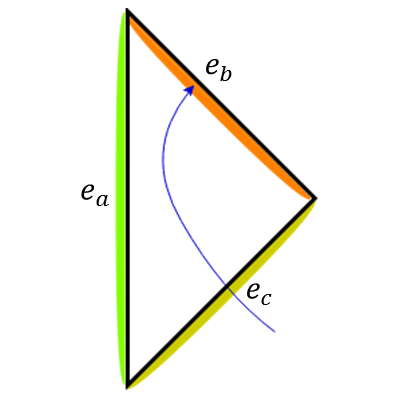
\includegraphics[width=0.49\columnwidth]{images/fail_propagate.png}}

	\caption[]{Two types of edges that are considered as area of crossing geodesic distance's path.}
	\label{fig:fig-two-type-edges}
\end{figure}


\subsection{Pseudo-sources of intervals from both sides}
\label{subsec:pseudo-sources laid on both side of adjacent faces}
The main idea of our approach is to detect areas where geodesic distance's paths are crossing together, like wave occlusion. Because we generate a cut graph so we define such areas as a set of edges.

First, we detect an edge $e_i$ whose intervals $I_{e_i}$ satisfy the condition: if there is an interval that $f_p$ is not same as other intervals then we consider $e_i \in \tilde{E}$. From figure \subref*{fig:geodesic_both_face}, we can see clearly that $e_a$ has two intervals $i_{e_{a,1}}$ and $i_{e_{a,2}}$, where first one has a pseudo-source from $f_l$ while second one has another pseudo-source from $f_r$. Typically, this kind of edges can be found a few in mesh (see figure \subref*{fig:edge from two faces}). 

\subsection{Non-propagation edge intervals}
\label{subsec:intervals fail to propagate}
Along with the edge type described in section \ref{subsec:pseudo-sources laid on both side of adjacent faces},  we need to define another edge type in cut graph. That is, this type of edges are nearby crossing geodesic distance's paths.

We detect an edge $e_i$ whose intervals $I_{e_i}$ satisfy the condition: all intervals have pseudo-sources from same face $f_p$ ($e_p$ can be different). Let opposite face be $f_{\bar{p}}$ and other two adjacent edges of $f_{\bar{p}}$ side be $e_{\bar{i}_1}$ and $e_{\bar{i}_2}$. We consider both $e_{\bar{i}_1}$ and $e_{\bar{i}_2}$ edges by the following condition.
\begin{itemize}
	\item Edge intervals have pseudo-sources from both sides (section \ref{subsec:pseudo-sources laid on both side of adjacent faces}).
	\item Edge intervals have $e_p \neq e_i$.
\end{itemize}

if both $e_{\bar{i}_1}$ and $e_{\bar{i}_2}$ match one of above conditions, then we consider $e_i \in \tilde{E}$. 

Considering an edge $e_a$ in figure \subref*{fig:geodesic_fail_propagte}, we can clearly see that edges $e_b$ and $e_c$ of opposite face $f_r$ ($e_{\bar{i}_1}$ and $e_{\bar{i}_2}$) have all intervals where their pseudo-sources are not on $e_a$ so we include $e_a$ into $\tilde{E}$. Vise-versa, when we are considering edge $e_c$; we can clearly see that edge $e_b$ has interval where its pseudo-source is on $e_c$ so we exclude $e_c$ from $\tilde{E}$.

Typically, this kind of edges can be found a lot in mesh and cover all areas of mesh (see figure \subref*{fig:edge nearby crossing}). Therefore, we need to eliminate unnecessary edges in $\tilde{E}$. Present state of cut graph looks similar to dangling edges in original one so we run the same iterative process to remove the valance-1 vertices in the graph. 

\begin{figure}[h!]
	\centering		
	\subfloat[\label{fig:edge from two faces}]{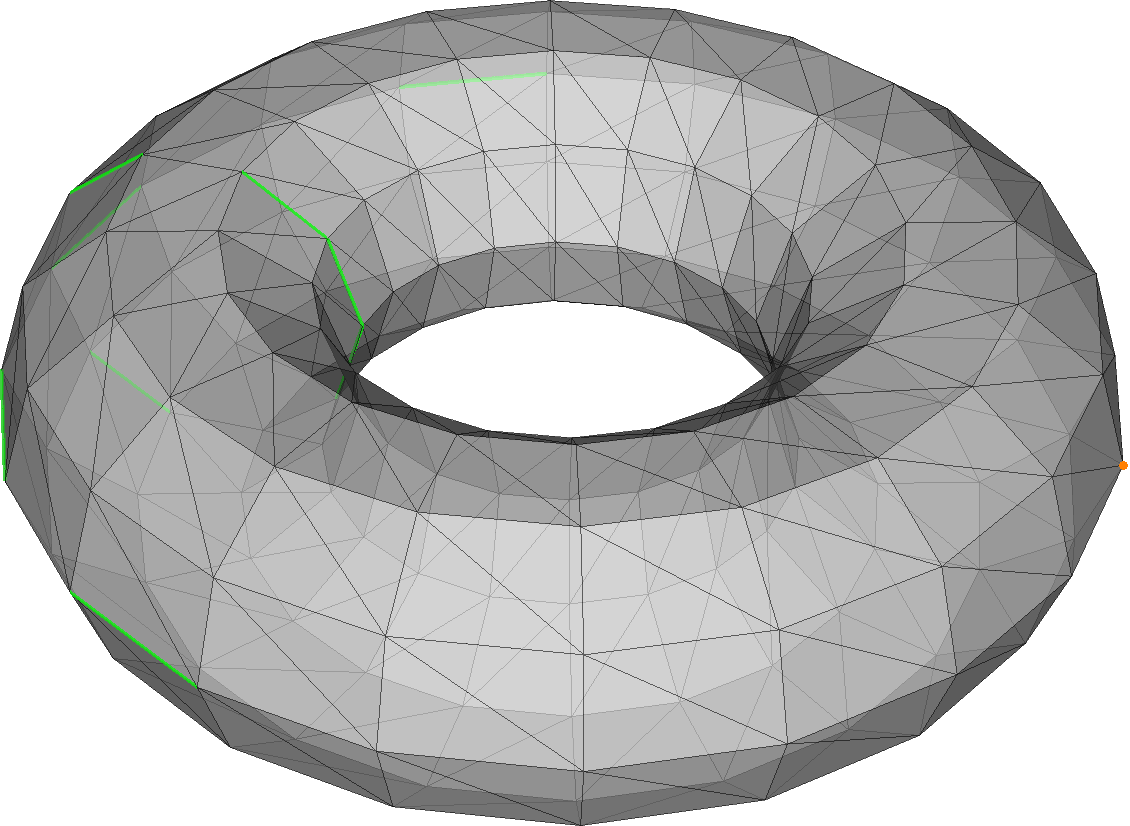
\includegraphics[width=0.48\columnwidth]{images/edge_two_faces.png}}
	\hspace{2pt}
	\subfloat[\label{fig:edge nearby crossing}]{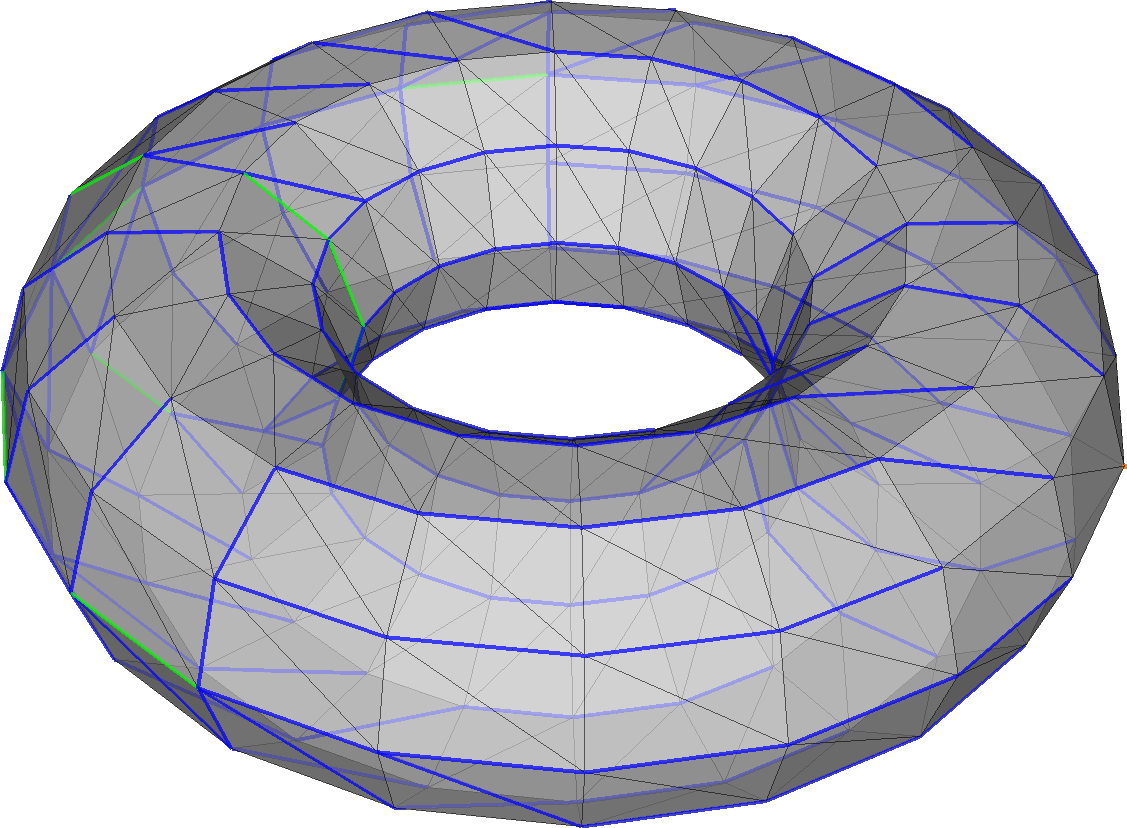
\includegraphics[width=0.48\columnwidth]{images/edge_nearby_crossing.png}}\\
	\subfloat[\label{fig:after truncate}]{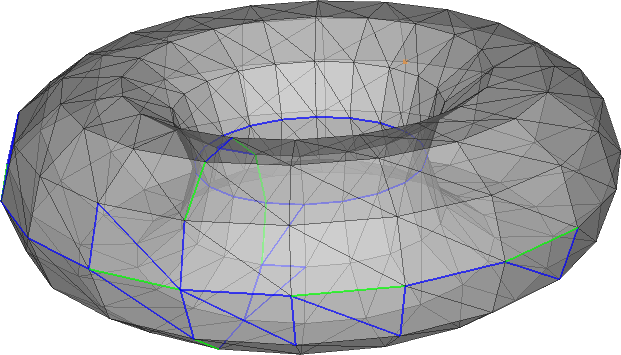
\includegraphics[width=0.75\columnwidth]{images/after_truncation.png}}\\
	\subfloat[\label{fig:neighbor edges}]{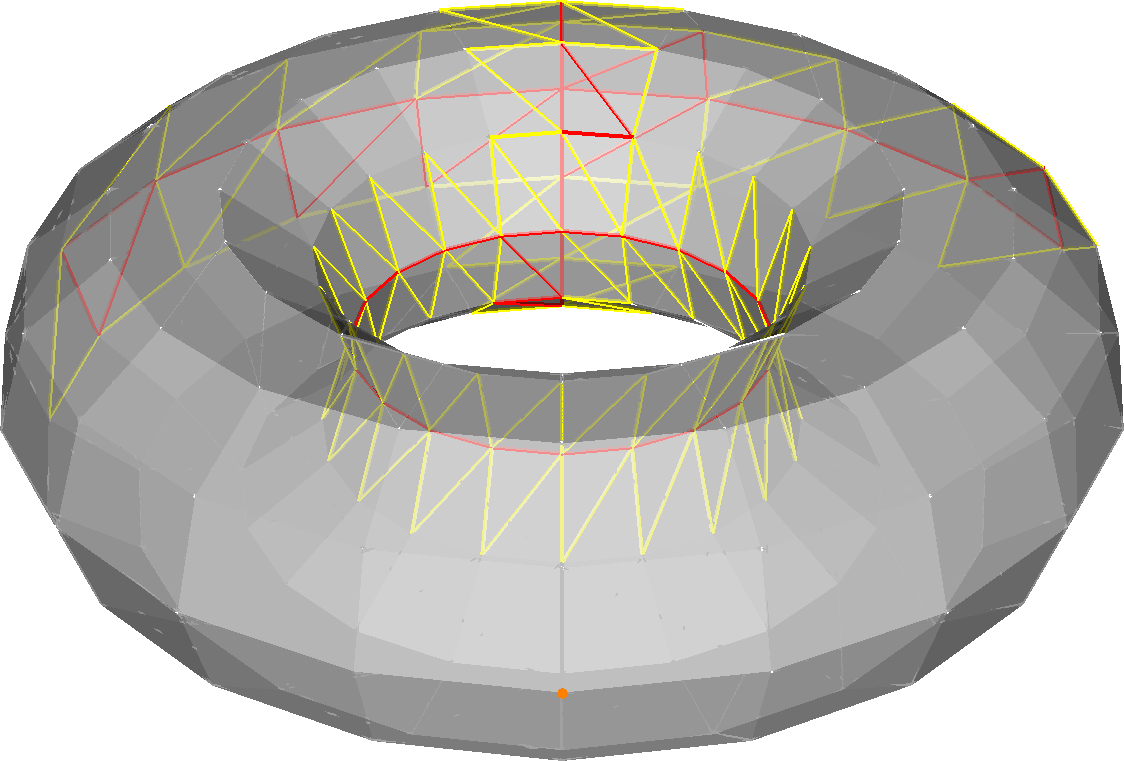
\includegraphics[width=0.75\columnwidth]{images/neighbor_edges.png}}	

	\caption[]{Processes to define $\tilde{E}$ and $\hat{E}$ on a torus model. \subref{fig:edge from two faces} shows green colored edges that their intervals' pseudo-sources are from both sides. \subref{fig:edge nearby crossing} shows blue colored edges that their intervals have not propagated. \subref{fig:after truncate} shows the graph after removing dangling edges. \subref{fig:neighbor edges} shows $\tilde{E}$ in red color and $\hat{E}$ in  yellow color.}
	\label{fig:fig-torus_edges_detected}
\end{figure}

\subsection{Ensure for non-separating cycles}
\label{subsec:ensure non-trivia}
After detecting in the set edges $\tilde{E}$ where geodesic distance's paths are crossing in section \ref{subsec:pseudo-sources laid on both side of adjacent faces} and \ref{subsec:intervals fail to propagate}, we aim to create a homotopy cut graph; non-separating and non-contractible cycles from $\tilde{E}$.

At this stage, $\tilde{E}$ may typically contains separating or contractible cycles (see figure \subref*{fig:after truncate}).  For separating cycles issue, we define all edges in $\hat{E}$ to be neighbors of each edges in $\tilde{E}$. We consider that a set of edges $\rho \equiv (\tilde{E} \cup \hat{E})$ contains $2g$ loops inside it.  

\subsection{Prioritize removing-edge queues}
After we ensured that $\rho$ contains $2g$ loops inside them, we try to create a valid cut graph along them. From this condition, we must eliminate edges that cause contractible cycles from $\rho$ and maintain non-separating property. Also, there are non-considered edges $\acute{E} \equiv (E - \rho)$ which we exclude from the cut graph.

One advantage of original method is to guarantee a valid cut graph when the propagation finished. Because of that, we used original one's propagation scheme. However, we want cut graph to be around $\tilde{E}$ as first priority and around $\hat{E}$ as second priority. Therefore, we altered the orders of removing edge in original propagation scheme. We created 3 removing-edge queues rather than single queue in original one. Each queue contains edges based on type of edges: 
$\acute{E}$, $\hat{E}$ and $\tilde{E}$.  And we mark each of them for low-to-high priority in the order of $\acute{E}$, $\hat{E}$ and $\tilde{E}$.

First, we remove faces around $v_s$ as seed triangles; similar to original one. Next, we iteratively analyze edges (adjacent only one triangle) in a non-empty queue under the conditions that we try to remove the edge and its adjacent face on low priority queue first and the edge with the shortest geodesic distance in the queue will be removed first.

After the propagation terminates and all queues become empty, the remaining edges contain $2g$ loops with non-separating and non-contractible properties. Again, we might shorten each loop for better quality in some further applications. At last, we generate a cut graph that enables to convert the mesh with genus $g$ into topological disk patch.


\section{\uppercase{Experimental Results}}
\label{sec:Experiment Results}
\noindent We tested the algorithms on a PC by using parameterization results from both original and our approach methods. We manually selected a vertex in input mesh to be $v_s$ then generate a cut graph. To create cut graphs from both methods with similar conditions, we want the both propagations to be spread out from same location. However, the original algorithm removes single seed triangle but our approach removes seed triangles around $v_s$. Therefore, we altered how to remove a seed triangle in original one to be same as our approach. With this alternation, it should not affect to overall performance in original one. Also, we applied shorten loops process after the propagation terminates.

After converting input mesh into disk topological patch, we applied stretch-minimizing parameterization from \cite{Yoshizawa_SMI04}.  We evaluated the parameterization results from both methods by using $L^2$ error (the root-mean-square stretch over all direction in planar domain) proposed by \cite{Sander:2001:TMP:383259.383307,Sander:2002:SP:581896.581909}.  

After experiments with the several mesh which genus $g \geq 1$, we noticed that original method and our approach can generate very similar or same cut graphs on asymmetry lookalike meshes in most cases. However on some symmetry shapes, cut graphs can be different from each others. Therefore, we selected some results which have noticeable difference on cut graphs between original and our approach, and do parameterizations.

As shown in Table \ref{table:result}, our approach can deliver lower  $L^2$ error than original one in most cases. There are some cases that original one has a large error value while our approach can deliver a small error.

\begin{table}[h]
	\setlength\extrarowheight{03pt}
	\caption{Experimental Results. Yellow and green cells indicate lower errors in comparison.}	
	\label{table:result} 
	\centering
	{\small 
	\begin{tabular}{|c|c|c|c|c|c|}
		
		\hline
	\multirow{2}{*}{case} & \multirow{2}{*}{genus} & \multicolumn{2}{ c|}{ square } & \multicolumn{2}{ c|}{ circular} \\\cline{3-6}
		         &       &   original &   our      &   original &   our\\
		\hline
		01    & 1  & 1.351   &  \cellcolor{yellow!25}1.335    &  1.493  &  \cellcolor{green!25}1.446 \\
		02    & 1  & 1.492   &  \cellcolor{yellow!25}1.468    &  1.687  &  \cellcolor{green!25}1.663 \\
		03    & 1  & \cellcolor{yellow!25}1.562   &  1.636    &  \cellcolor{green!25}1.800  &  2.102 \\
		04    & 1  & 1.551   &  \cellcolor{yellow!25}1.417    &  2.011  &  \cellcolor{green!25}1.635 \\
		05    & 1  & 1.561   &  \cellcolor{yellow!25}1.362    &  1.924  &  \cellcolor{green!25}1.538 \\
		06    & 2  & 1.667   &  \cellcolor{yellow!25}1.466    &  2.246  &  \cellcolor{green!25}1.701 \\
		07    & 2  & \cellcolor{yellow!25}1.390   &  1.442    &  1.603  &  \cellcolor{green!25} 1.554 \\
		08    & 3  & 1.457   &  \cellcolor{yellow!25}1.452    &  1.688  &  \cellcolor{green!25}1.679 \\
		09    & 3  & 2.041   &  \cellcolor{yellow!25}2.025    &  \cellcolor{green!25}9.279  &  9.827 \\
		10   & 3  & 471.2   &  \cellcolor{yellow!25}1.509    &  4.068  &  \cellcolor{green!25}1.978 \\
		11   & 3  & 939.2   &  \cellcolor{yellow!25}1.625    &  6.348  &  \cellcolor{green!25}4.115 \\
		12   & 3  & 221.3K   &  \cellcolor{yellow!25}79.9K    &  383.2K  &  \cellcolor{green!25}203.4K \\
		\hline		
	\end{tabular}}
\end{table}

We show the visual results from our experiments in figure \ref{fig:experiment results}. Note that all meshes do not contain any holes and case 02-03, 04-05, 06-07 and 08-09 are same models with different $v_s$ location.

\section{\uppercase{Conclusions}}
\label{sec:conclusion}

\noindent We have presented an enhancement method to generate a cut graph in high-genus surface for homotopy cutting. Cut graph is generated based on an exact geodesic distance theory, by detecting areas where geodesic distance's paths are crossing together. We show how to detect these areas into a set of edges by analyzing edges' intervals. Then, we show how to ensure non-separating and non-contractible cycles by including neighbor edges into the set and applying original approach with minor adjustments in propagation queues. We can generate equally or more suitable edge-graph than original method while keeping similar performance and stability as original one.

An open topic of this propagation scheme is, it still requires manual starting location of propagation (seed triangle or $v_s$ in our approach). The quality of cut graph is dependency on user specific position.  To generate an optimal cut graph on a high genus surface, it is better to have shortest cut loop where it pass through on each surface's handle. Therefore, it is interesting topic for how to define starting location of propagation $v_s$ that generate optimal cut graph.


\section*{\uppercase{Acknowledgements}}
\noindent The images in figure \ref{fig:gim figure} and \ref{fig:fig-original_genus_reducing_process}  are from \cite{Gu:2002:GI:566654.566589} paper and presentation file. Models are courtesy of the AIM@SHAPE repository. Special thanks are given to Danil Kirsanov for exact geodesic distance code, to Shin Yoshizawa for parameterization code and to the anonymous reviewers for comments and suggestions.
This study is supported by JSPS KAKENHI (Grant Number 24300035).



\bibliographystyle{apalike}
{\small
\bibliography{genus_cutting}}
\vfill

\begin{figure*}[th!]
	\centering	
	\captionsetup[subfigure]{labelformat=empty}
	\subfloat[\label{fig:case01}case 01]{ \centering	
		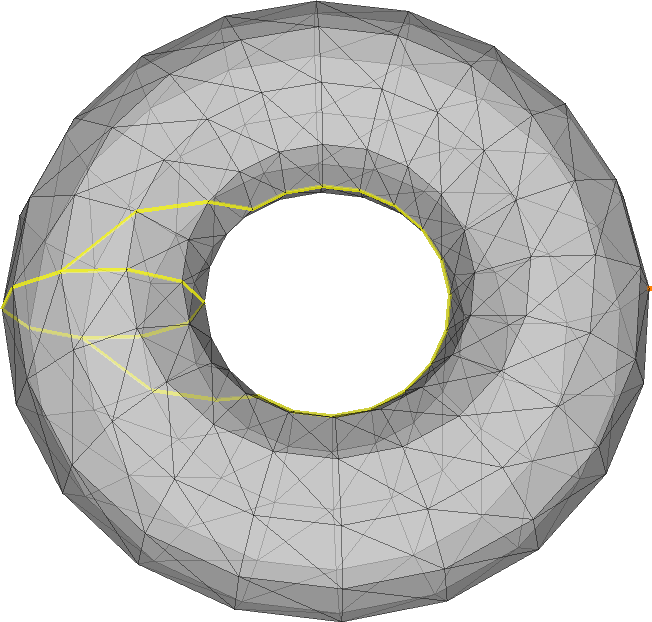
\includegraphics[width=0.35\columnwidth]{images/experiment/test01/original.png}\hspace{8pt} 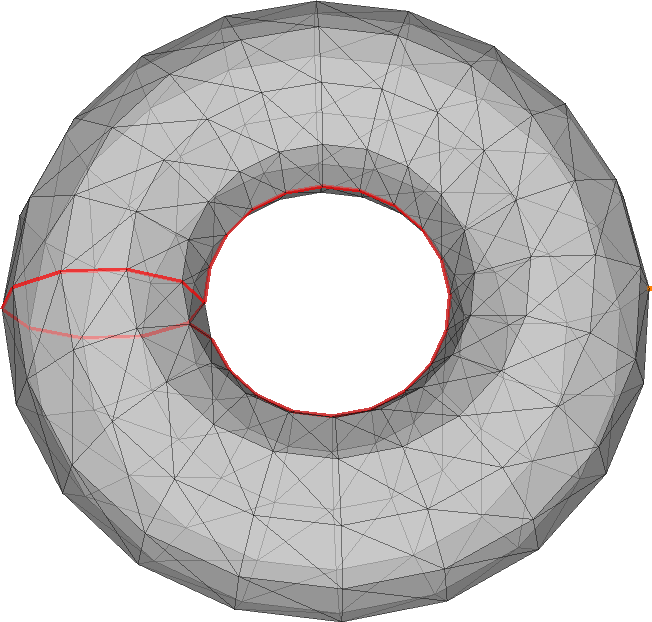
\includegraphics[width=0.35\columnwidth]{images/experiment/test01/propose.png}
	}
	\hspace{20pt}
	\subfloat[\label{fig:case02}case 02]{ \centering
		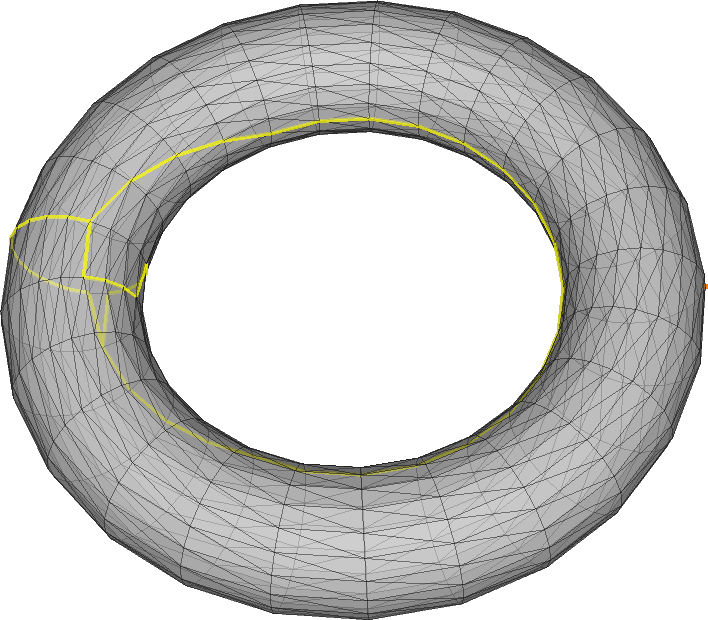
\includegraphics[width=0.35\columnwidth]{images/experiment/test02/original.png}\hspace{8pt} 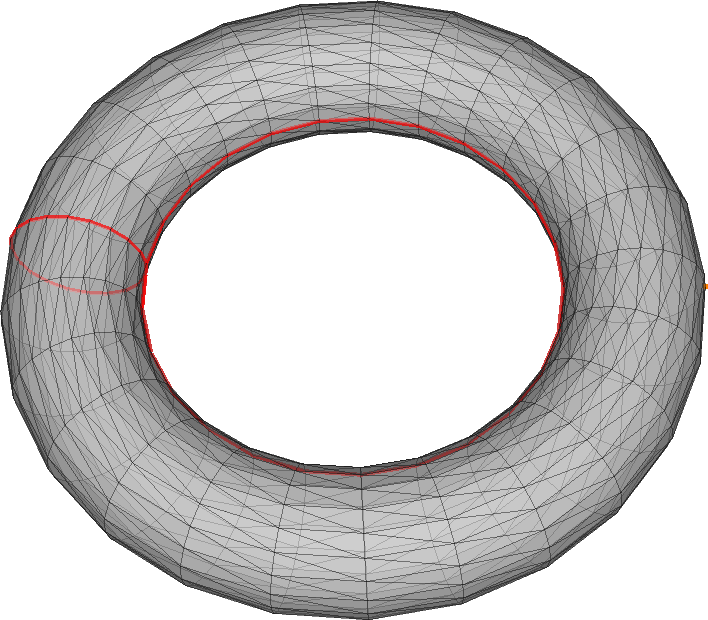
\includegraphics[width=0.35\columnwidth]{images/experiment/test02/propose.png}
	}\\
	
	\subfloat[\label{fig:case03}case 03]{ \centering
		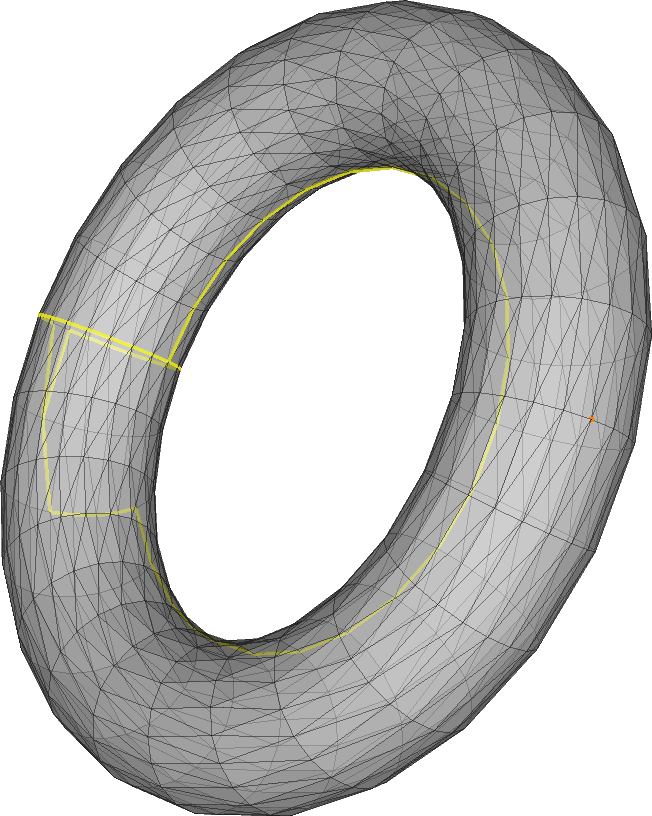
\includegraphics[width=0.33\columnwidth]{images/experiment/test03/original.png}\hspace{8pt} 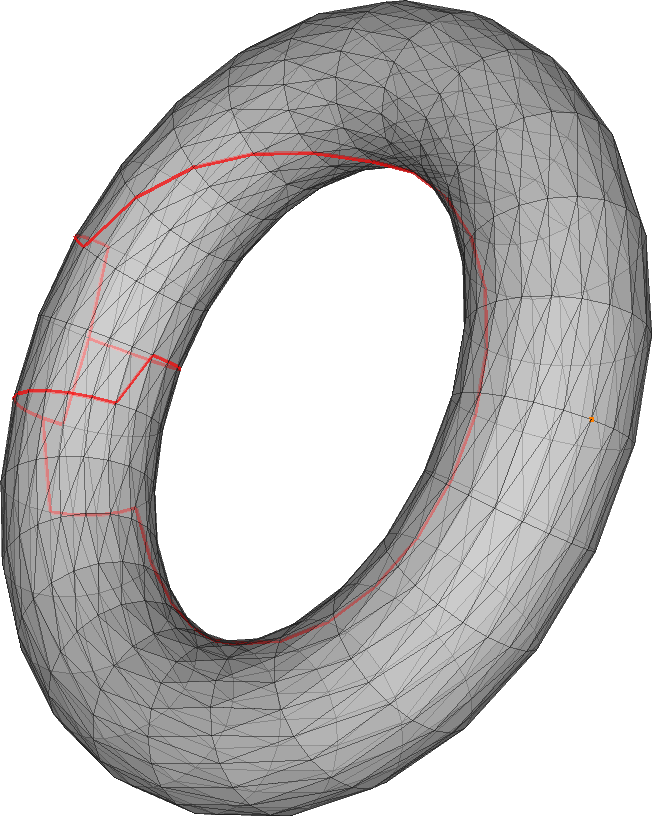
\includegraphics[width=0.33\columnwidth]{images/experiment/test03/propose.png}
	}
	\hspace{20pt}
	\subfloat[\label{fig:case04}case 04]{ \centering
		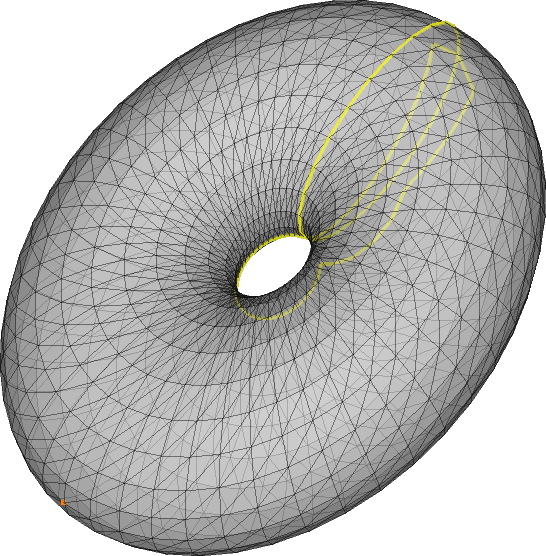
\includegraphics[width=0.35\columnwidth]{images/experiment/test04/original.png}\hspace{8pt} 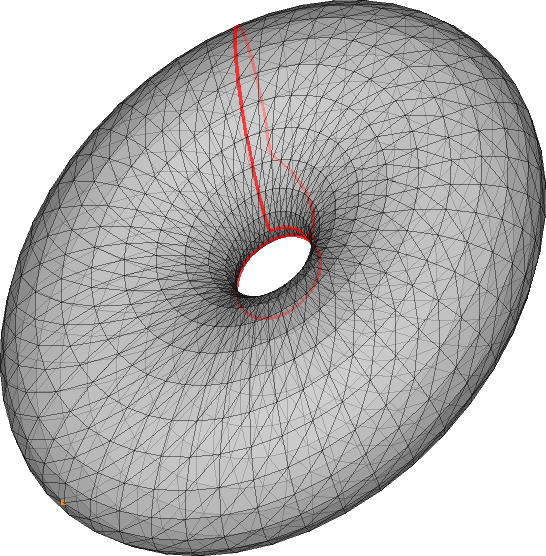
\includegraphics[width=0.35\columnwidth]{images/experiment/test04/propose.png}
	}\\
	
	\subfloat[\label{fig:case05}case 05]{ \centering
		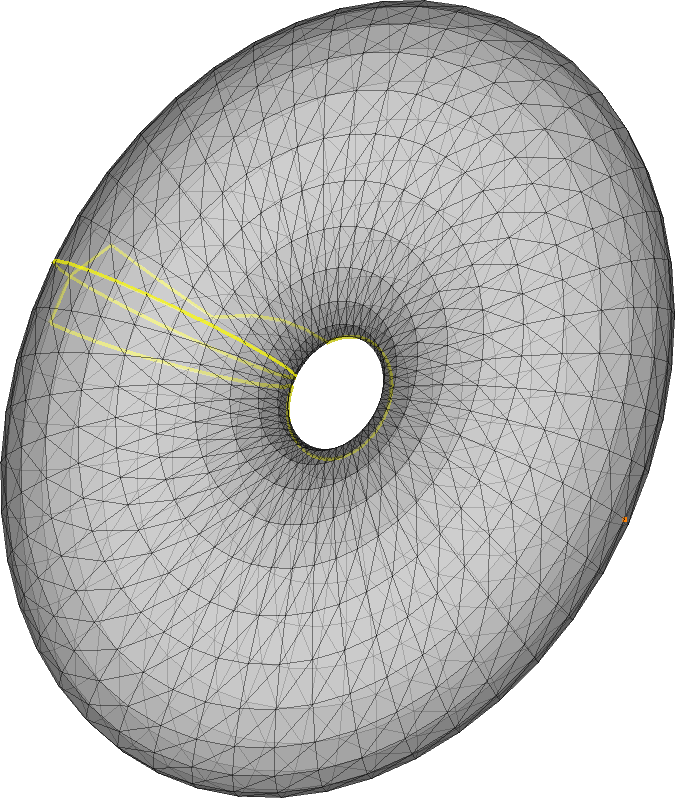
\includegraphics[width=0.35\columnwidth]{images/experiment/test05/original.png}\hspace{8pt} 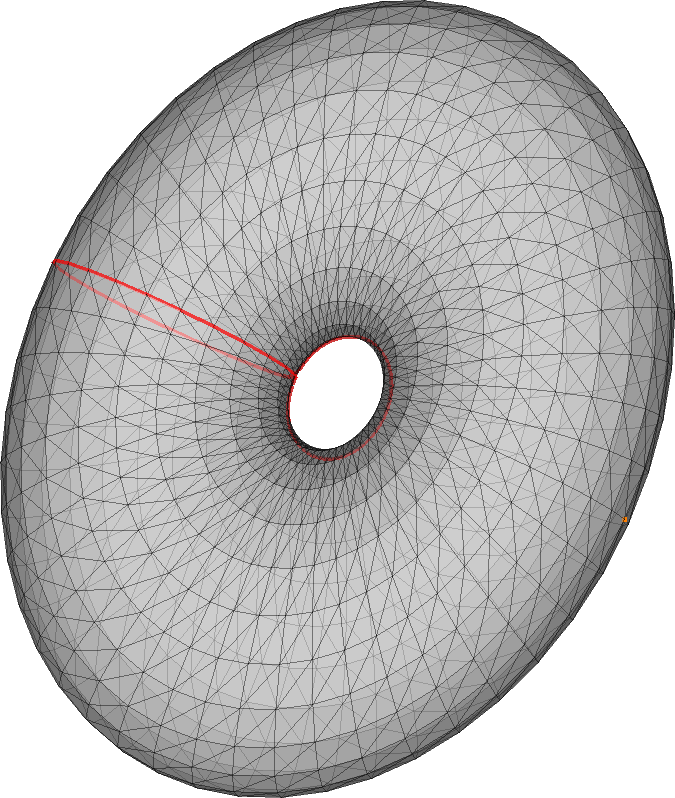
\includegraphics[width=0.35\columnwidth]{images/experiment/test05/propose.png}
	}
	\hspace{20pt}
	\subfloat[\label{fig:case06}case 06]{ \centering
		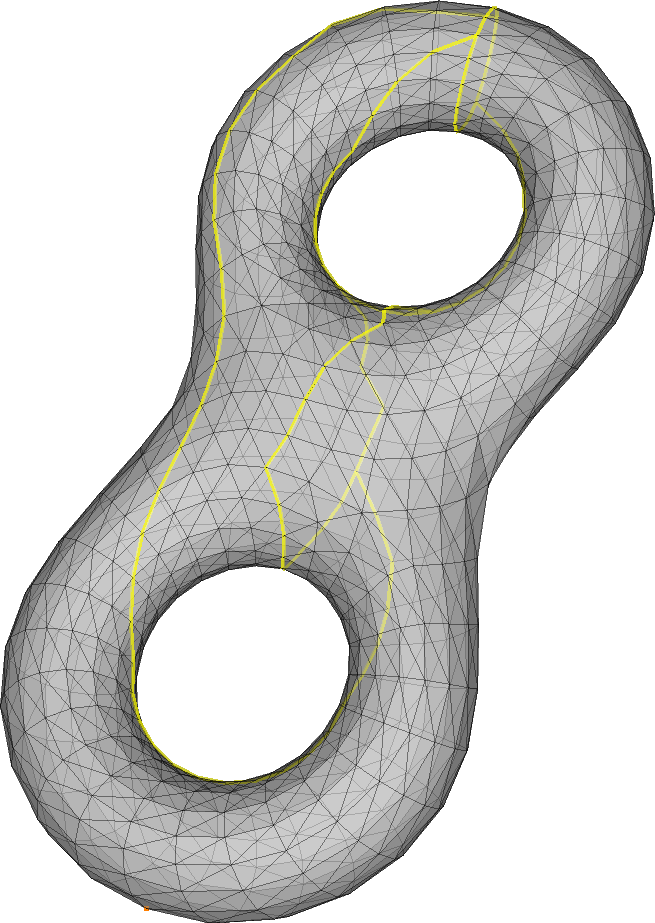
\includegraphics[width=0.33\columnwidth]{images/experiment/test06/original.png}\hspace{8pt} 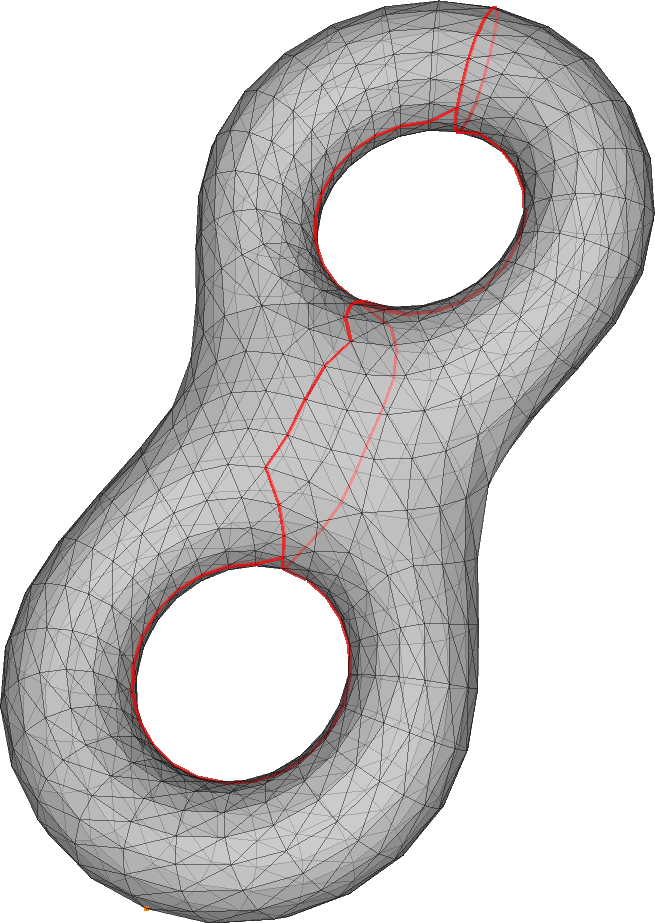
\includegraphics[width=0.33\columnwidth]{images/experiment/test06/propose.png}
	}\\

	\subfloat[\label{fig:case07}case 07]{ \centering
		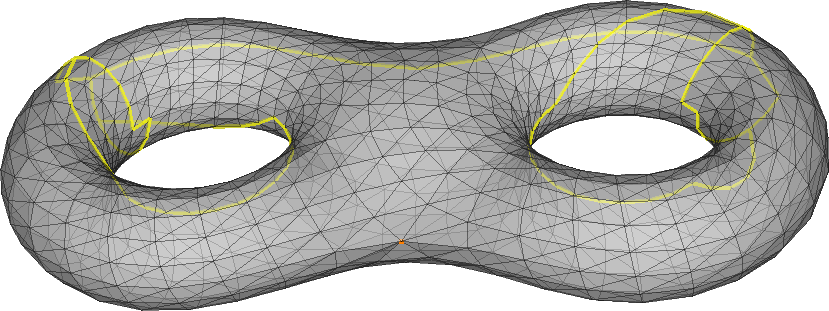
\includegraphics[width=0.4\columnwidth, angle=45]{images/experiment/test07/original.png}
		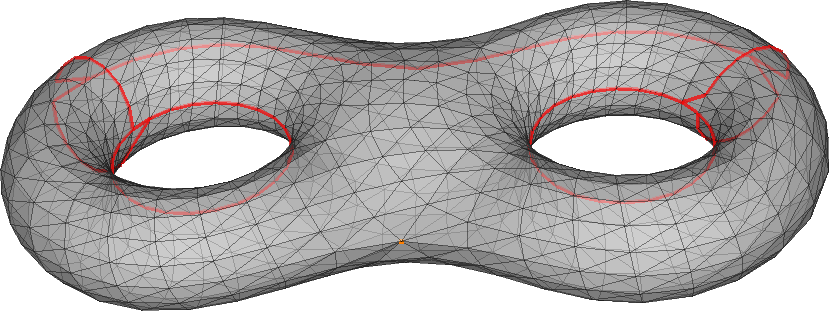
\includegraphics[width=0.4\columnwidth, angle=45]{images/experiment/test07/propose.png}
	}
	\hspace{20pt}
	\subfloat[\label{fig:case08}case 08]{
		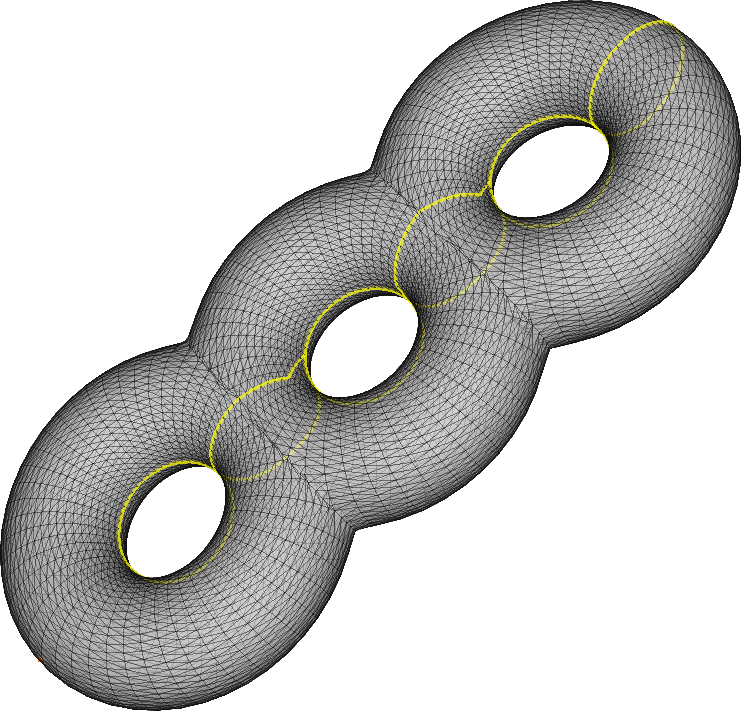
\includegraphics[width=0.35\columnwidth]{images/experiment/test08/original.png}\hspace{8pt} 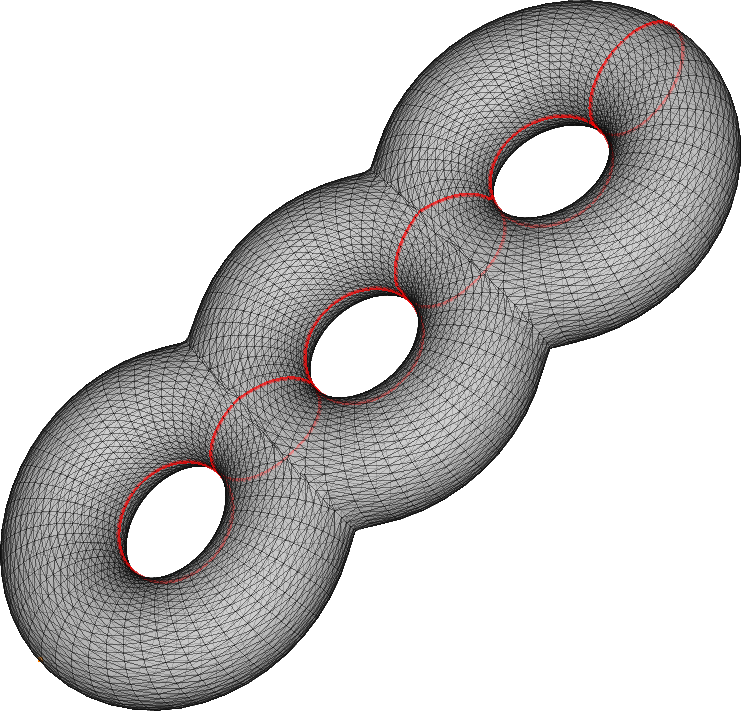
\includegraphics[width=0.35\columnwidth]{images/experiment/test08/propose.png}
	}\\


	\subfloat[\label{fig:case09}case 09]{ \centering
		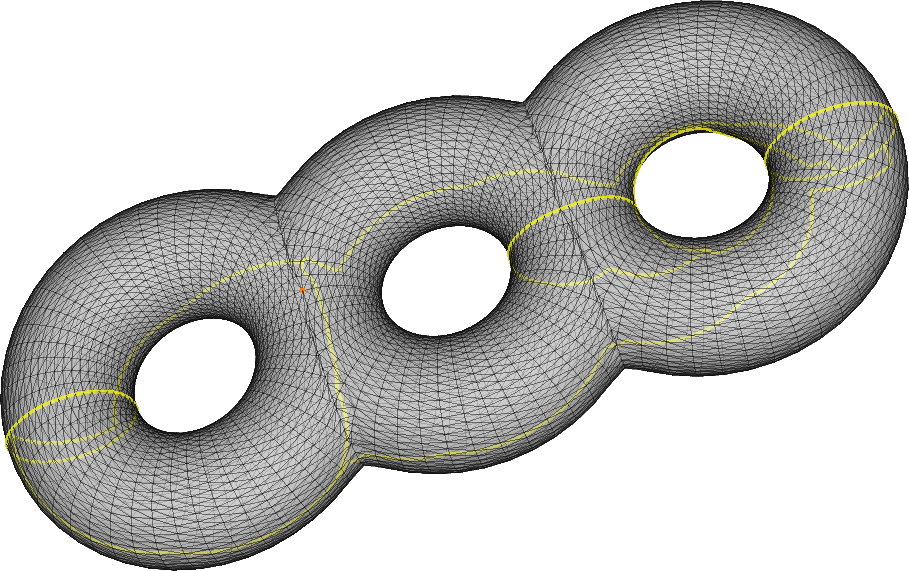
\includegraphics[width=0.35\columnwidth]{images/experiment/test09/original.png} \hspace{8pt}
		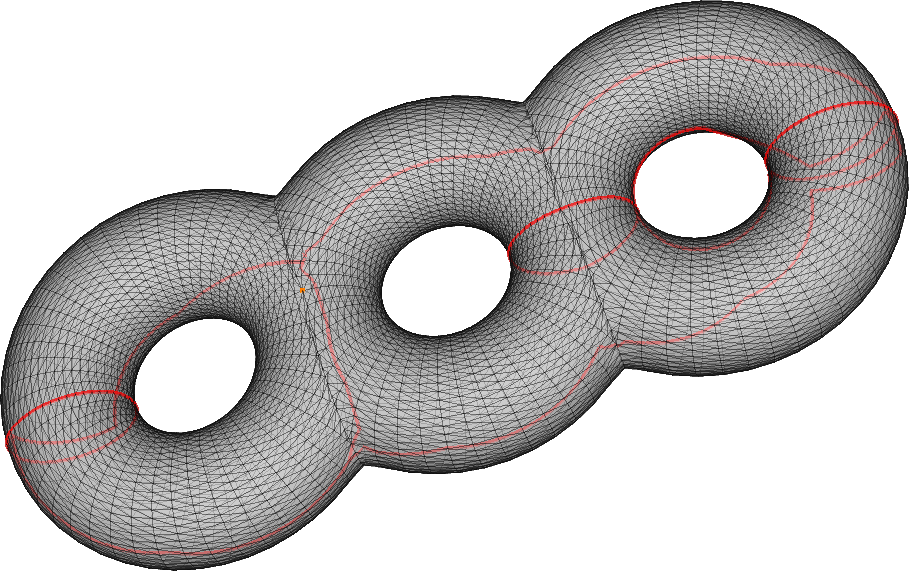
\includegraphics[width=0.35\columnwidth]{images/experiment/test09/propose.png}
	}
	\hspace{20pt}
	\subfloat[\label{fig:case10}case 10]{ \centering
		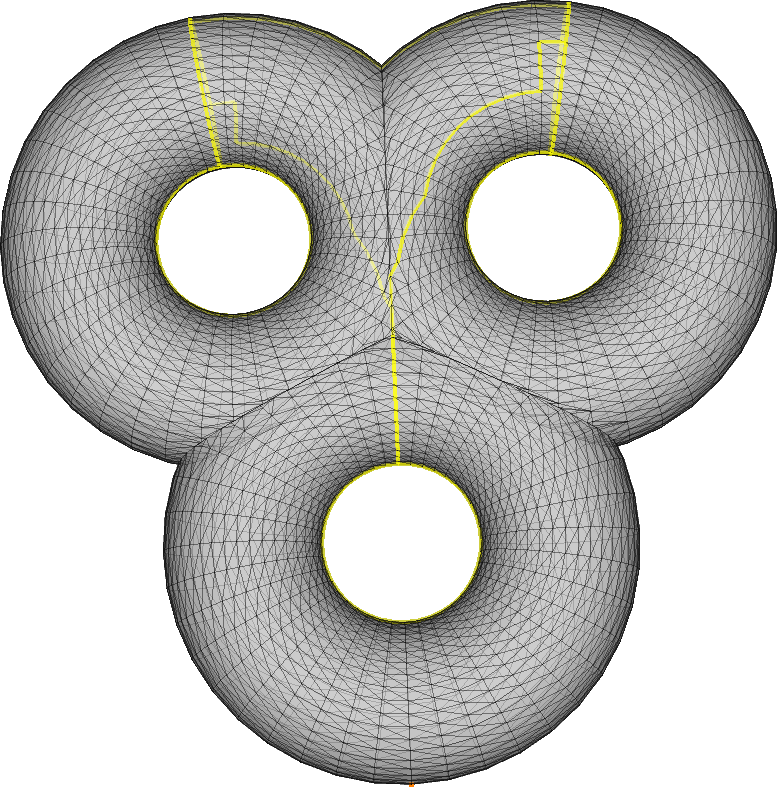
\includegraphics[width=0.35\columnwidth]{images/experiment/test10/original.png}\hspace{8pt} 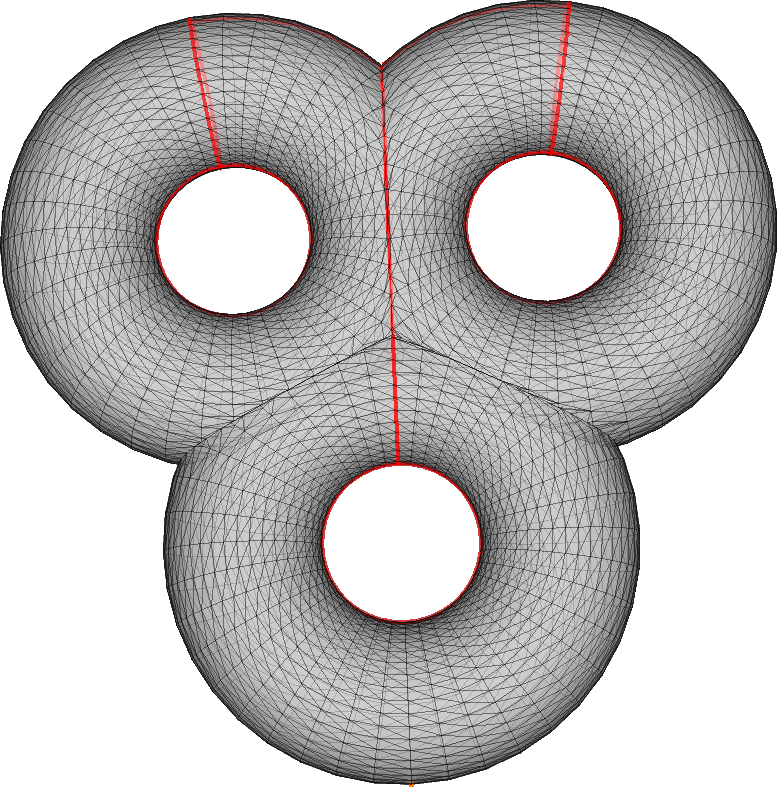
\includegraphics[width=0.35\columnwidth]{images/experiment/test10/propose.png}
	}\\

	\subfloat[\label{fig:case11}case 11]{ \centering
		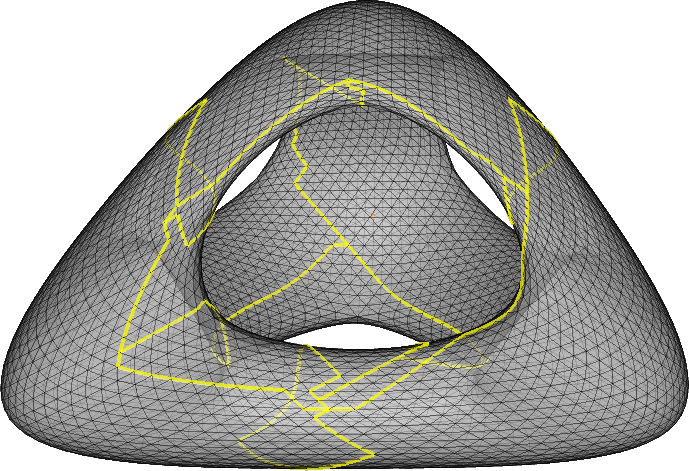
\includegraphics[width=0.35\columnwidth]{images/experiment/test11/original.png}\hspace{8pt} 
		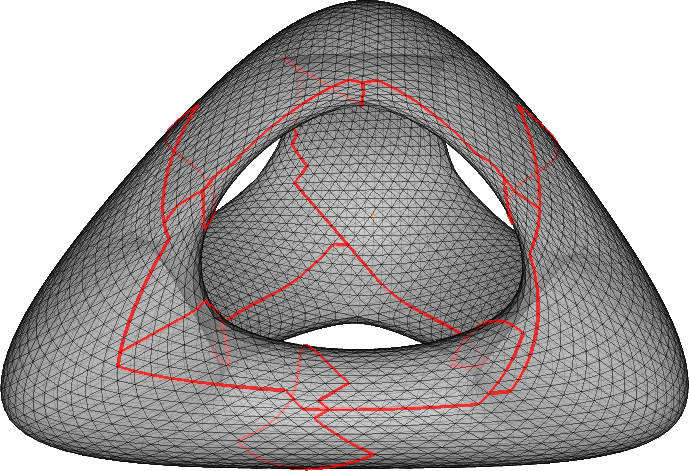
\includegraphics[width=0.35\columnwidth]{images/experiment/test11/propose.png}
	}
	\hspace{20pt}
	\subfloat[\label{fig:case12}case 12]{ \centering
		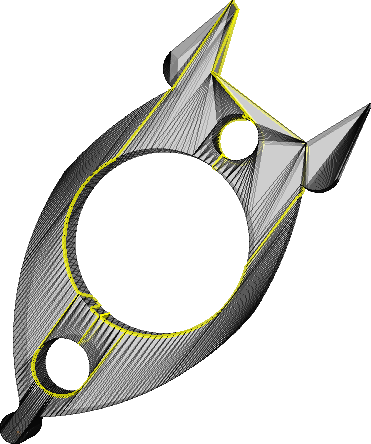
\includegraphics[width=0.35\columnwidth]{images/experiment/test12/original.png}\hspace{8pt} \includegraphics[width=0.35\columnwidth]{images/experiment/test12/propose.png}
	}\\
	\caption[]{Results of homotopy cutting from original (geometry images) and our approach methods. The meshes having yellow line are original approach results. The meshes having red line are our approach results.}
	\label{fig:experiment results}
\end{figure*}

\end{document}

